% =====================================================================
%  YILDIZ TEKNİK ÜNİVERSİTESİ - FEN-EDEBİYAT FAKÜLTESİ
%  LİSANS BİTİRME TEZİ (KL-058 / FR-1925 yazım kılavuzuna uyarlanmıştır)
%  Bu dosya otomatik olarak makale kaynağından üretilmiştir.
% =====================================================================
\documentclass[12pt,a4paper]{report}

% --- Karakter kodlaması ve Türkçe ---
\usepackage[T1]{fontenc}
\usepackage[utf8]{inputenc}
\IfFileExists{glyphtounicode.tex}{\input{glyphtounicode}\pdfgentounicode=1}{}
\IfFileExists{cmap.sty}{\usepackage{cmap}}{}
\usepackage[shorthands=off,turkish]{babel}

% --- Times New Roman benzeri yazı tipi (metin + matematik) ---
\usepackage{mathptmx}

% --- Sayfa düzeni: sol 3,5 cm; diğer kenarlar 2,5 cm ---
\usepackage[a4paper,left=3.5cm,right=2.5cm,top=2.5cm,bottom=2.5cm]{geometry}

% --- 1,5 satır aralığı ---
\usepackage{setspace}
\onehalfspacing

% --- Matematik ---
\usepackage{amsmath,amssymb,amsfonts,mathrsfs,mathtools}
\numberwithin{equation}{chapter}
\allowdisplaybreaks
\setlength{\jot}{4pt}

% --- Grafik + renk ---
\usepackage{graphicx}
\graphicspath{{figures/}{thesis/figures/}}
\usepackage[dvipsnames]{xcolor}

% --- Çizelgeler ---
\usepackage{booktabs}
\usepackage{array}
\usepackage{tabularx}
\usepackage{float}
\usepackage{placeins}

% --- Listeler, kod, TikZ ---
\usepackage{enumitem}
\usepackage{microtype}
\usepackage{listings}
\usepackage{needspace}
\usepackage{tikz}
\usetikzlibrary{calc,positioning,arrows.meta,decorations.pathreplacing,
                decorations.markings,matrix,fit,backgrounds,shapes.misc}
\emergencystretch=3em

% --- Teoremler ---
\usepackage{amsthm}

% --- Başlık biçimlendirme (titlesec): 1. derece 17,5pt, 2. derece 14pt ---
\usepackage{titlesec}
\titleformat{\chapter}[hang]
  {\normalfont\fontsize{17.5}{21}\bfseries}{\thechapter}{12pt}{}
\titlespacing*{\chapter}{0pt}{0pt}{18pt}
\titleformat{\section}
  {\normalfont\fontsize{14}{17}\bfseries}{\thesection}{10pt}{}
\titlespacing*{\section}{0pt}{14pt}{8pt}
\titleformat{\subsection}
  {\normalfont\fontsize{12}{15}\bfseries}{\thesubsection}{8pt}{}
\setcounter{secnumdepth}{3}
\setcounter{tocdepth}{2}
% \paragraph run-in başlıkları içindekiler'i kirletmesin: numarasız + toc'a yazılmaz
\titleformat{\paragraph}[runin]{\normalfont\normalsize\bfseries}{}{0pt}{}
\titlespacing*{\paragraph}{0pt}{6pt}{1em}
\AtBeginDocument{\setcounter{tocdepth}{2}}
\makeatletter
\renewcommand{\l@paragraph}[2]{}% paragraf düzeyini içindekiler'den tamamen çıkar
\makeatother

% --- Şekil / çizelge başlıkları: numaradan sonra nokta yerine boşluk ---
\usepackage{caption}
\captionsetup{labelsep=space,font=small,justification=centering,
              singlelinecheck=true}
\captionsetup[table]{skip=4pt}
% Numaralandırmada son rakamdan sonra nokta yok
\renewcommand{\thechapter}{\arabic{chapter}}
\renewcommand{\thesection}{\thechapter.\arabic{section}}
\renewcommand{\thesubsection}{\thesection.\arabic{subsection}}
\renewcommand{\thefigure}{\thechapter.\arabic{figure}}
\renewcommand{\thetable}{\thechapter.\arabic{table}}
\renewcommand{\theequation}{\thechapter.\arabic{equation}}

% --- "Çizelge" terminolojisi (YTÜ FBE) ---
\addto\captionsturkish{%
  \renewcommand{\tablename}{Çizelge}%
  \renewcommand{\figurename}{Şekil}%
  \renewcommand{\contentsname}{İÇİNDEKİLER}%
  \renewcommand{\listfigurename}{ŞEKİL LİSTESİ}%
  \renewcommand{\listtablename}{ÇİZELGE LİSTESİ}%
  \renewcommand{\bibname}{KAYNAKLAR}%
  \renewcommand{\appendixname}{EK}%
}

% --- Sayfa numarası alt-ortada ---
\usepackage{fancyhdr}
\fancypagestyle{plain}{%
  \fancyhf{}\renewcommand{\headrulewidth}{0pt}%
  \fancyfoot[C]{\thepage}%
}
\pagestyle{plain}

% --- Listing renk paleti ---
\definecolor{codebg}{RGB}{248,248,248}
\definecolor{codeframe}{RGB}{210,210,210}
\definecolor{codekeyword}{RGB}{120,40,140}
\definecolor{codestring}{RGB}{40,110,40}
\definecolor{codecomment}{RGB}{90,90,90}

\lstdefinestyle{pyblock}{
    language=Python,
    basicstyle=\ttfamily\footnotesize,
    keywordstyle=\bfseries\color{codekeyword},
    stringstyle=\color{codestring},
    commentstyle=\itshape\color{codecomment},
    backgroundcolor=\color{codebg},
    frame=single,
    rulecolor=\color{codeframe},
    framerule=0.4pt,
    numbers=left,
    numberstyle=\tiny\color{gray},
    stepnumber=1,
    numbersep=8pt,
    showstringspaces=false,
    breaklines=true,
    breakatwhitespace=true,
    breakindent=0pt,
    postbreak=\mbox{\textcolor{codeframe}{hookrightarrow}\space},
    columns=fullflexible,
    keepspaces=true,
    tabsize=4,
    literate={-}{{\char`\-}}1,
    xleftmargin=1.5em,
    xrightmargin=0.5em,
    framexleftmargin=1em,
    aboveskip=0.9em,
    belowskip=0.9em,
    captionpos=b,
}
\lstdefinestyle{bashblock}{
    language=bash,
    basicstyle=\ttfamily\small,
    backgroundcolor=\color{codebg},
    frame=single,
    rulecolor=\color{codeframe},
    framerule=0.4pt,
    numbers=none,
    showstringspaces=false,
    breaklines=true,
    columns=fullflexible,
    keepspaces=true,
    literate={-}{{\char`\-}}1,
    xleftmargin=1.5em,
    xrightmargin=0.5em,
    framexleftmargin=1em,
    aboveskip=1.4em,
    belowskip=0.9em,
    captionpos=b,
}
\lstset{style=pyblock}
\renewcommand{\lstlistingname}{Kod}

% --- Accent renkleri (TikZ) ---
\definecolor{accent}{RGB}{59,91,146}
\definecolor{accentsoft}{RGB}{155,180,216}
\definecolor{oddsign}{RGB}{138,40,132}

% --- Hyperref ---
\usepackage[hidelinks]{hyperref}
\usepackage{url}

% --- Teorem ortamları (Türkçe) ---
\theoremstyle{plain}
\newtheorem{theorem}{Teorem}[chapter]
\newtheorem{proposition}[theorem]{Önerme}
\newtheorem{lemma}[theorem]{Lemma}
\newtheorem{corollary}[theorem]{Sonuç}
\theoremstyle{definition}
\newtheorem{definition}[theorem]{Tanım}
\newtheorem{example}[theorem]{Örnek}
\newtheorem{remark}[theorem]{Not}
\renewcommand{\proofname}{Kanıt}

% --- Matematik makroları ---

% --- TikZ ortak stilleri ---
\tikzset{
  strand/.style={line width=1pt, accent!80!black},
  rbox/.style={draw=accent!70!black, fill=accentsoft!55, rounded corners=2pt,
               line width=0.8pt, minimum height=6mm},
  rdot/.style={circle, fill=accent, inner sep=1.6pt},
  knode/.style={circle, draw=accent!70!black, fill=accentsoft!45,
                line width=0.8pt, minimum size=7mm, font=\small},
  kedge/.style={accent!70!black, line width=0.9pt},
  faredge/.style={oddsign!75!black, line width=0.9pt, densely dashed},
  glabel/.style={font=\footnotesize, accent!60!black},
}

% Kapakta kullanılacak başlık bilgileri
\newcommand{\TezBaslik}{Quantum Grup Yapılarının Python Ortamında Modellenmesi}
\newcommand{\TezBaslikEN}{Modelling Quantum Group Structures in a Python Environment}
\newcommand{\Ogrenci}{Taha Berk TEREKLİ}
\newcommand{\OgrenciNo}{Öğrenci No: 22025083}
\newcommand{\Danisman}{Prof.\ Dr.\ Salih ÇELİK}
\newcommand{\Bolum}{Matematik Bölümü}
\newcommand{\TarihAy}{Haziran}
\newcommand{\TarihYil}{2026}

\begin{document}

% ======================= DIŞ KAPAK =======================
\begin{titlepage}

\begin{center}

\includegraphics[width=7cm]{figures/ytu_logo.png}\\[1.2cm]
{\large\bfseries T.C.}\\[2pt]
{\large\bfseries YILDIZ TEKNİK ÜNİVERSİTESİ}\\[2pt]
{\large\bfseries FEN-EDEBİYAT FAKÜLTESİ}\\[2pt]
{\large\bfseries MATEMATİK BÖLÜMÜ}\\[2.2cm]

{\fontsize{16}{20}\selectfont\bfseries \TezBaslik}\\[2.2cm]

{\large \Ogrenci}\\[2pt]
{\large \OgrenciNo}\\[2.2cm]

{\large\bfseries LİSANS BİTİRME TEZİ}\\[2.2cm]

{\large Danışman}\\[2pt]
{\large \Danisman}\\[2.6cm]

{\large \TarihAy, \TarihYil}
\end{center}

\end{titlepage}

% ======================= İÇ KAPAK =======================
\pagenumbering{roman}
\setcounter{page}{1} % i (numara basılmaz)
\thispagestyle{empty}

\begin{center}

\includegraphics[width=7cm]{figures/ytu_logo.png}\\[1.2cm]
{\large\bfseries T.C.}\\[2pt]
{\large\bfseries YILDIZ TEKNİK ÜNİVERSİTESİ}\\[2pt]
{\large\bfseries FEN-EDEBİYAT FAKÜLTESİ}\\[2pt]
{\large\bfseries MATEMATİK BÖLÜMÜ}\\[2.2cm]

{\fontsize{16}{20}\selectfont\bfseries \TezBaslik}\\[2.2cm]

{\large \Ogrenci}\\[2pt]
{\large \OgrenciNo}\\[2.2cm]

{\large\bfseries LİSANS BİTİRME TEZİ}\\[2.2cm]

{\large Danışman}\\[2pt]
{\large \Danisman}\\[2.6cm]

{\large \TarihAy, \TarihYil}
\end{center}

\clearpage

% ======================= ÖNSÖZ =======================
\thispagestyle{empty} % ii (numara basılmaz)
\chapter{ÖNSÖZ}
\addcontentsline{toc}{chapter}{ÖNSÖZ}

Bu çalışma, modern matematiksel fiziğin ve cebirsel yapıların kesişiminde yer alan
kuantum grupları, bilgisayar destekli sembolik hesaplamayla buluşturma çabasının
bir ürünüdür. Amaç, kuantum grup Uq(sl2) ve kuantum süpergrup GLq(2|1) için temel
temsil-teorik ve Yang--Baxter tipi bağıntıları, elle yürütüldüğünde uzun ve hataya
açık olan hesapları, açık kaynaklı, test edilebilir ve yeniden üretilebilir bir
Python altyapısına taşımaktır.

Tez konusunun belirlenmesinde ve çalışmanın her aşamasında değerli bilgi, deneyim
ve yönlendirmelerini esirgemeyen, GLq(2|1) kuantum süpergrubunun kurucularından
biri olarak bu alandaki engin birikimini benimle paylaşan danışmanım
Sayın \Danisman'e en içten teşekkürlerimi sunarım. Ayrıca eğitim hayatım boyunca
maddi ve manevi desteklerini benden hiçbir zaman esirgemeyen aileme şükranlarımı
borç bilirim.

\vspace{1.5cm}
\begin{flushright}
\Ogrenci\\
\TarihAy, \TarihYil
\end{flushright}
\clearpage

% ======================= İÇİNDEKİLER =======================
\renewcommand{\contentsname}{İÇİNDEKİLER}
\tableofcontents
\clearpage

% ======================= SİMGE LİSTESİ =======================
\chapter{SİMGE LİSTESİ}
\addcontentsline{toc}{chapter}{SİMGE LİSTESİ}

\noindent
\begin{tabularx}{\textwidth}{@{}p{3.2cm}X@{}}
Uq(sl2) & Drinfeld--Jimbo kuantum grubu \\
sl2 & İz sıfır 2×2 matrislerin Lie cebri \\
U(g) & Evrensel sarmalayıcı cebir \\
E, F, K, K^-1 & Uq(sl2)'nin üreteçleri \\
q & Deformasyon parametresi \\
[n]q & q-tamsayı, (q^n-q^-n)/(q-q^-1) \\
Vn & (n+1)-boyutlu indirgenemez temsil \\
v0 & En yüksek ağırlık vektörü \\
Δ & Eş-çarpım (comultiplication) \\
ε & Eş-birim (counit) \\
S & Antipot \\
R & R-matrisi \\
Ř & Örgülü R-matrisi, Ř=τ R \\
τ & Takas (permütasyon) operatörü \\
⊗ & Tensör çarpımı \\
GLq(2|1) & Kuantum süpergrup \\
p(ei) & ei baz vektörünün paritesi (derecesi) \\
P & Süper permütasyon matrisi \\
Rij & Tensör kuvvetinde i,j faktörlerine yerleşen R \\
B(n) & Vn'nin kristal tabanı \\
zeta & İlkel birim kök \\
\end{tabularx}

\clearpage

% ======================= KISALTMA LİSTESİ =======================
\chapter{KISALTMA LİSTESİ}
\addcontentsline{toc}{chapter}{KISALTMA LİSTESİ}

\noindent
\begin{tabularx}{\textwidth}{@{}p{3.2cm}X@{}}
CG    & Clebsch--Gordan \\
QYBE  & Kuantum Yang--Baxter Denklemi (Quantum Yang--Baxter Equation) \\
RTT   & R T1 T2 = T2 T1 R inşa yöntemi \\
SI    & Uluslararası Birim Sistemi \\
YBE   & Yang--Baxter Denklemi (Yang--Baxter Equation) \\
YTÜ   & Yıldız Teknik Üniversitesi \\
\end{tabularx}

\clearpage

% ======================= ŞEKİL LİSTESİ =======================
\listoffigures
\addcontentsline{toc}{chapter}{ŞEKİL LİSTESİ}
\clearpage

% ======================= ÇİZELGE LİSTESİ =======================
\listoftables
\addcontentsline{toc}{chapter}{ÇİZELGE LİSTESİ}
\clearpage

% ======================= ÖZET =======================
\chapter{ÖZET}
\addcontentsline{toc}{chapter}{ÖZET}
\begin{center}
{\bfseries \TezBaslik}\\[4pt]
\Ogrenci\\[8pt]
\Bolum\ Lisans Bitirme Tezi\\[6pt]
Danışman: \Danisman\\[10pt]
\end{center}

Bu tez, Drinfeld--Jimbo kuantum grubu Uq(sl2) ve GLq(2|1) kuantum süpergrubu için
temel temsil-teorik ve Yang--Baxter tipi bağıntıları Python/SymPy ortamında yeniden
üretilebilir biçimde modellemektedir. Yöntemin çekirdeği, her cebirsel eşitliği açık
sonlu boyutlu temsiller üzerinde bir kalıntı matrisine indirgemek ve bu matrisin tüm
girdilerini sembolik olarak sadeleştirerek sıfır olup olmadığını denetlemektir.

Uq(sl2) için sonlu boyutlu en yüksek ağırlıklı Vn temsilleri açık matrislerle
kurulmuş; tanımlayıcı bağıntılar, Hopf yapısı, tensör çarpımı eylemi ve
Clebsch--Gordan en yüksek ağırlık vektörleri seçilen temsiller üzerinde sembolik
olarak doğrulanmıştır. V1⊗ V1 üzerinde R-matrisi, kuantum Yang--Baxter
denklemi, örgü bağıntısı ve Hecke skein özdeşliği sıfır-kalıntı yöntemiyle kontrol
edilmiştir. GLq(2|1) tarafında ise literatürde verilen 9× 9 R-matrisi
bağımsız olarak kodlanmış, p(e1)=p(e2)=0, p(e3)=1 parite konvansiyonu ile
süper permütasyon kullanılarak R13 yerleşimi kurulmuş ve graded Yang--Baxter
kalıntısının tüm 27× 27 girdilerinin sıfır olduğu sembolik olarak
doğrulanmıştır. Sonuçların her biri \texttt{pytest} tabanlı testlere bağlanmıştır.
Çalışmanın temel katkısı yeni bir kuantum grup tanımı vermek değil, bilinen kuantum
grup ve kuantum süpergrup yapılarını modüler, test edilebilir ve yeniden
üretilebilir bir sembolik doğrulama altyapısına dönüştürmektir.

\vspace{0.6cm}
\noindent\textbf{Anahtar Kelimeler:} kuantum gruplar, Uq(sl2),
kuantum süpergruplar, GLq(2|1), Yang--Baxter denklemi, sembolik hesaplama.
\clearpage

% ======================= ABSTRACT =======================
\chapter{ABSTRACT}
\addcontentsline{toc}{chapter}{ABSTRACT}
\begin{center}
{\bfseries \TezBaslikEN}\\[4pt]
\Ogrenci\\[8pt]
Department of Mathematics, Undergraduate Thesis\\[6pt]
Advisor: \Danisman\\[10pt]
\end{center}

This thesis models, in a reproducible way within the Python/SymPy environment, the
fundamental representation-theoretic and Yang--Baxter type relations of the
Drinfeld--Jimbo quantum group Uq(sl2) and the quantum supergroup GLq(2|1). The core
of the method is to reduce every algebraic identity to a residual matrix on explicit
finite-dimensional representations and, by symbolically simplifying every entry of
this matrix, to check whether it vanishes.

For Uq(sl2), the finite-dimensional highest-weight representations Vn are built with
explicit matrices; the defining relations, the Hopf structure, the tensor product
action and the Clebsch--Gordan highest-weight vectors are verified symbolically on
selected representations. On V1⊗ V1, the R-matrix, the quantum
Yang--Baxter equation, the braid relation and the Hecke skein identity are checked by
the zero-residual method. On the GLq(2|1) side, the 9× 9 R-matrix given in
the literature is encoded independently; using the parity convention
p(e1)=p(e2)=0, p(e3)=1 and a super permutation, the placement R13 is
constructed and all 27× 27 entries of the graded Yang--Baxter residual are
shown to be symbolically zero. Each result is tied to \texttt{pytest}-based tests. The
main contribution is not to introduce a new quantum group but to turn known quantum
group and quantum supergroup structures into a modular, testable and reproducible
symbolic verification infrastructure.

\vspace{0.6cm}
\noindent\textbf{Keywords:} quantum groups, Uq(sl2), quantum
supergroups, GLq(2|1), Yang--Baxter equation, symbolic computation.
\clearpage

% ======================= ANA METİN =======================
\pagenumbering{arabic}
\setcounter{page}{1}

\chapter{Giriş}

Kuantum gruplar, 1980'lerin ortasında V.~Drinfeld ve M.~Jimbo'nun~\cite{Drinfeld,Jimbo,KS} --- istatistik
mekaniğin integrallenebilir modellerini ve bunların temelinde yatan
\emph{kuantum Yang--Baxter denklemini} cebirsel bir dile oturtma çabası içinde ---
birbirinden bağımsız olarak vardığı yapılardır. Adlarındaki ``grup'' sözcüğü
yanıltıcıdır: kuantum gruplar birer Lie grubu değildir. Daha çok, evrensel
sarmalayıcı cebir U(g)'nin bir q parametresi boyunca tek-parametreli
deformasyonu olan ve ne değişmeli ne de eş-değişmeli (cocommutative) olan
\emph{Hopf cebirleridir}. Bu deformasyonun kalbinde, örgülü monoidal
kategorilerde iki nesnenin tutarlı biçimde yer değiştirmesini kodlayan, böylece
integrallenebilir sistemlerle düğüm değişmezlerini aynı çatı altında buluşturan
Yang--Baxter denklemi ve onun çözümü olan R-matrisi durur.

Bu denklemlerin somut temsiller üzerinde sağlandığını göstermek, q'ya bağlı
yüksek boyutlu matris çarpımlarını gerektirir; el ile yürütüldüğünde işlem hem
uzar hem de hataya açık hâle gelir. Burada izlenen yol, söz konusu cebirsel
manipülasyonları sembolik bilgisayar cebiriyle (Python/SymPy) modellemek, her
bağıntıyı bir sıfır-kalıntı matris testine indirgemek ve elde edilen sonuçları
otomatik birim testlere bağlamaktır. Anlatı iki eksende ilerler: \textbf{(i)}
Uq(sl2) için temsil teorisi ve R-matrisi altyapısı; \textbf{(ii)} GLq(2|1)
kuantum süpergrubu için graded Yang--Baxter doğrulaması.

Bu iki eksen, kuantum grupların prototipi Uq(sl2) ile Salih Çelik ve Sultan A.\ Çelik'in tanıttığı
GLq(2|1) kuantum süpergrubunu beş doğrulama başlığı altında ele alan ortak bir
hedefte buluşur:
\begin{enumerate}[leftmargin=*]
  \item \textbf{Cebirsel}: dört tanımlayıcı bağıntının ve dokuz Hopf
        aksiyomunun (eş-birleşmelilik, eş-birim, antipot) matris düzeyinde
        sembolik doğrulanması.
  \item \textbf{Temsil teorik}: (n+1)-boyutlu indirgenemez temsil Vn'in
        açık inşası, Vm ⊗ Vn Clebsch--Gordan ayrışımının q-deforme
        katsayılarıyla hesaplanması.
  \item \textbf{Topolojik}: V1⊗ V1 üzerinde R-matrisinin
        inşası, kuantum Yang--Baxter denkleminin ve örgü bağıntısının
        sembolik matris doğrulaması; bu doğrulamanın düğüm değişmezleri (Jones
        polinomu) ile bağlantısı.
  \item \textbf{Asimptotik}: q parametresinin üç farklı limitinde aynı
        temsilin yapısının nasıl değiştiğinin somut karşılaştırılması.
  \item \textbf{Süpergrup ve graded YBE}: Salih Çelik ve Sultan A.\ Çelik tarafından tanımlanan
        GLq(2|1) kuantum süpergrubunun 9× 9 R-matrisi kodlanarak,
        graded Yang--Baxter denklemi 27× 27 matris düzeyinde sembolik
        olarak doğrulanır.
\end{enumerate}

Bu çalışmanın özgün katkısı, yeni bir kuantum grup tanımlamak değildir.
Katkı, literatürde bilinen Uq(sl2) ve GLq(2|1) yapılarını sonlu boyutlu
temsiller üzerinde yeniden üretilebilir, test edilebilir ve sembolik bir
doğrulama altyapısına dönüştürmektir. Bu kapsamda Uq(sl2) temsilleri, tanımlayıcı
bağıntılar, Hopf aksiyomları, tensör çarpımları, Clebsch--Gordan en yüksek
ağırlık vektörleri, R-matrisi kontrolleri ve limit karşılaştırmaları aynı
paket içinde ele alınır. Ayrıca Salih Çelik ve Sultan A.\ Çelik'in
GLq(2|1) için verdiği R-matrisi bağımsız olarak kodlanır ve graded
Yang--Baxter denklemi, parite uyumlu R13 yerleşimiyle 27× 27
matris girdileri düzeyinde doğrulanır. Raporlanan her sembolik eşitlik,
\texttt{pytest} tabanlı yeniden çalıştırılabilir bir teste bağlanır.

Çalışmanın yazılım ayağı, yalnızca SymPy'ye bağımlı ve modüler olarak
tasarlanmış \texttt{quantum\_group} adlı Python paketidir; her doğrulama
\texttt{pytest} testleriyle otomatik biçimde yeniden çalıştırılabilir. Böylece raporlanan her eşitlik, ilgili
testi koşturan herkes tarafından bağımsızca yeniden üretilebilir.

\paragraph{Tezin akışı.} İlkin gerekli teorik zemin --- gruplar, Lie
cebirleri, Hopf cebirleri, Uq(sl2) ve temsiller --- yoğun ama eksiksiz biçimde
verilir. Ardından yazılım mimarisi tanıtılır. Sonraki bölümler hesaplamalı
katkıları sırayla sunar: Clebsch--Gordan ayrışımı, Uq(sl2) için R-matrisi ve
YBE, GLq(2|1) için graded Yang--Baxter doğrulaması ve üç asimptotik limit.
Kapanış bölümü bulguları toparlayıp ileri çalışma yönlerini sıralar.

\chapter{Teorik Arka Plan}

Aşağıda, kuantum grupların üzerine kurulduğu klasik cebirsel zemin --- gruplar,
Lie cebirleri, evrensel sarmalayıcı cebir ve Hopf yapısı --- ele alınır.
Anlatım bilinçli olarak sıkıştırılmıştır; ancak ilerideki bölümler için gereken
hiçbir kavram atlanmamış, vurgu sl2 → Uq(sl2) → Vn hattını izleyen bir
çizgide tutulmuştur.

\section{Gruplar, Lie Cebirleri ve Evrensel Sarmalayıcı Cebir}

\paragraph{Tanım 2.1.}
Bir \emph{grup} G, birleşmeli bir ikili işlem · : G × G → G,
iki yanlı bir birim eleman e ∈ G ve her elemanın bir tersi olan bir
küme yapısıdır.


Sürekli simetri grupları üzerinde diferansiyel hesap yapabilmek için Lie
gruplarına geçilir: G aynı zamanda düzgün bir manifolddur ve grup
işlemleri düzgündür. Klasik örnekler GLn(C), SLn(C),
SOn, SUn'dur. Bir Lie grubunun \emph{infinitezimal}
yapısı tanjant uzayında saklıdır.

\paragraph{Tanım 2.2.}
Bir cisim K üzerinde bir \emph{Lie cebri} g, antisimetrik ve Jacobi
özdeşliğini sağlayan iki-doğrusal [ · , · ] : g × g → g
parantezi ile donatılmış vektör uzayıdır:
\[
  [x,y] = -[y,x], \qquad
  [x,[y,z]] + [y,[z,x]] + [z,[x,y]] = 0.
\]


Matris Lie grupları için Lie parantezi komütatördür: [x,y] = xy - yx.
Lie grup ile Lie cebir arasındaki köprü üstel dönüşüm exp : g → G ile
verilir. Lie cebrinin temsil teorisini lineerleştiren araç, bir sonraki
adımdır.

\paragraph{Tanım 2.3.}
g bir Lie cebri olsun. \emph{Evrensel sarmalayıcı cebir} U(g),
g'yi içeren ve xy - yx = [x,y] bağıntısı dışında hiçbir bağıntıya
tabi olmayan birleşmeli birimli cebirdir.


g'nin temsilleri ile U(g)'nin temsilleri kanonik olarak birebir
karşılık gelir; ve kuantum gruba deformasyon hedefimiz tam olarak U(g)
nesnesidir, g'nin kendisi değil.

\section{sl2 Lie Cebri}

İz sıfır 2 × 2 kompleks matrisleri vektör uzayı sl2(C) üç
boyutludur ve standart bazı:
\[
  e = \begin{pmatrix} 0 & 1 \\ 0 & 0 \end{pmatrix},\qquad
  f = \begin{pmatrix} 0 & 0 \\ 1 & 0 \end{pmatrix},\qquad
  h = \begin{pmatrix} 1 & 0 \\ 0 & -1 \end{pmatrix}.
\]
Bu eleman üçlüsü temel bağıntıları sağlar:
\begin{equation}\label{eq:sl2-rels}
  [h,e] = 2e, \qquad [h,f] = -2f, \qquad [e,f] = h.
\end{equation}
Küçük boyutuna karşın sl2, yarı-basit Lie cebirlerinin tüm yapı
taşıdır: her böyle cebir basit kökler tarafından indekslenmiş sl2
kopyalarından dokunmuş gibidir.

\paragraph{Teorem 2.4 (sl2'nin sonlu boyutlu temsilleri).}
sl2(C)'nin sonlu boyutlu indirgenemez temsilleri, negatif olmayan
tamsayı n ∈ Z≥q 0 ile birebir karşılık gelir. Vn adlı temsil
(n+1)-boyutludur, baz v0, v1, ..., vn üzerinde
\[
  h \cdot v_k = (n - 2k) v_k, \quad
  f \cdot v_k = v_{k+1}, \quad
  e \cdot v_k = k(n-k+1)\, v_{k-1},
\]
ve sınır koşulları f · vn = 0, e · v0 = 0.


h'nin özdeğerleri olan n - 2k tamsayılarına \emph{ağırlıklar} denir;
bu, kuantum gruba geçişte K-özdeğerleri olarak yeniden ortaya çıkacaktır.

\section{Hopf Cebirleri}

Bir cebir verildiğinde, onun temsilleriyle ne yapabileceğimiz tek başına çarpım
yapısıyla belirlenmez. İki temsilin tensör çarpımının yine bir temsil olması,
trivial (skaler) bir temsilin tanımlanabilmesi ve her temsile bir dual
eşlik edebilmesi --- bunların hiçbiri birleşmeli çarpımdan kendiliğinden çıkmaz.
Eksik olan, cebire eklenen üç ek dönüşümdür: bir elemanı iki kopyaya ``dağıtan''
eş-çarpım, skalere indirgeyen eş-birim ve tersleme rolünü üstlenen antipot. Bu
üçlü \emph{Hopf cebir} aksiyomlarını oluşturur ve aslında temsil teorisinin
tensör/dual işlemlerini cebirin içine gömme aracıdır.

\paragraph{Tanım 2.5.}
K cismi üzerinde birleşmeli birimli bir cebir H, eğer eş-çarpım
Δ : H → H ⊗ H, eş-birim ε : H → K ve antipot
S : H → H dönüşümleriyle donatılmış ve aşağıdakileri sağlıyorsa
\emph{Hopf cebri}'dir:
\begin{enumerate}[leftmargin=*]
  \item (Δ ⊗ id) circ Δ = (id ⊗ Δ) circ Δ \quad (eş-birleşmelilik)
  \item (ε ⊗ id) circ Δ = id = (id ⊗ ε) circ Δ \quad (eş-birim)
  \item mu circ (S ⊗ id) circ Δ = ε( · ) 1 = mu circ (id ⊗ S) circ Δ \quad (antipot)
\end{enumerate}
Burada mu cebir çarpımıdır; ayrıca Δ ve ε cebir homomorfizmleri,
S cebir anti-homomorfizmi olmak zorundadır.


Hopf yapısının temsil teorik anlamı kritiktir:
\begin{itemize}[leftmargin=*]
  \item İki temsil V, W verildiğinde, V ⊗ W üzerinde H-etkisi
        eş-çarpım aracılığıyla tanımlanır: X · (v ⊗ w) := Δ(X) · (v ⊗ w).
  \item Eş-birim ε, trivial temsil K'ya karşılık gelir.
  \item Antipot S, dual temsil V^*'ı tanımlamak için kullanılır.
\end{itemize}

\paragraph{Örnek 2.6.}
Her U(g), eş-değişmeli (cocommutative) bir Hopf cebridir; üreteçler
x ∈ g üzerinde
\[
  \Delta(x) = x \otimes 1 + 1 \otimes x, \quad \varepsilon(x) = 0, \quad S(x) = -x.
\]
Eş-değişme, klasik tensör çarpımının değişmeli olmasının cebirsel
karşılığıdır. Kuantum grupta tam olarak bu özellik bozulacaktır.


\chapter{Kuantum Grup Uq(sl2)'nin Tanımı}

Drinfeld--Jimbo fikrinin özü, U(sl2)'nin Serre tipi bağıntılarını ayakta
tutarken Cartan üretecini bir grup-benzeri öğeye dönüştürmektir. Klasik
h yerine tersinir bir K = q^h değişkeni konur; bu sayede Cartan eylemi
``q üssü'' biçiminde köşegenleşir ve [e,f]=h bağıntısı, [h]q
ifadesiyle yumuşatılmış bir versiyona geçer. Deformasyon parametresi q, ayrı
bir cebirsel nicelik eklemez; var olan tüm yapı sabitlerini q'nun rasyonel
fonksiyonlarına taşır ve q→ 1 limitinde her şeyi klasik U(sl2)'ye geri
indirir.

Bu çalışmada q çoğunlukla formel bir parametre olarak ele alınır ve sembolik
hesaplamalar Q(q) üzerinde yürütülür. Bir karmaşık değere özelleştirme
yapıldığında q∈C^× ve tanımda görünen paydalar için q≠ pm 1
varsayılır; birim köklerde ise temsil teorisinin değiştiği ayrıca
Bölüm~10 içinde belirtilir.

\paragraph{Tanım 3.1.}\label{def:Uq}
Uq(sl2) kuantum grubu, Q(q) üzerinde dört üreteç E, F, K, K^-1
ile aşağıdaki bağıntılara tabi birleşmeli cebirdir:
\begin{align}
  K K^{-1} &= K^{-1} K = 1, \tag{R1} \\
  K E K^{-1} &= q^{2} E, \tag{R2} \\
  K F K^{-1} &= q^{-2} F, \tag{R3} \\
  [E, F] := EF - FE &= \frac{K - K^{-1}}{q - q^{-1}}. \tag{R4}
\end{align}


Bu cebir bir Hopf cebridir; üreteçler üzerinde:
\begin{align}
  \Delta(E) &= E \otimes 1 + K \otimes E, \\
  \Delta(F) &= F \otimes K^{-1} + 1 \otimes F, \\
  \Delta(K) &= K \otimes K, \\
  \varepsilon(E) &= \varepsilon(F) = 0, \quad \varepsilon(K) = 1, \\
  S(E) &= -K^{-1} E, \quad S(F) = -F K, \quad S(K) = K^{-1}.
\end{align}
Burada Δ eş-\emph{değişmeli değildir}: τ circ Δ ≠ Δ (bunu
örgülü R-matrisin varlığı tam olarak kuantize edecek).

\section{q-Deformasyon Sezgisi}

q-tamsayılar şu formülle tanımlanır:
\begin{equation}\label{eq:qint}
  [n]_q := \frac{q^n - q^{-n}}{q - q^{-1}} = q^{n-1} + q^{n-3} + \dots + q^{-(n-1)}.
\end{equation}
L'H{\^o}pital kuralıyla bakıldığında q→ 1 için [n]q→ n olur; benzer
biçimde q-faktöriyel [n]q! = [n]q[n-1]q·s[1]q klasik
n!'e yaklaşır. Burada kritik olan nokta şudur: [n]q yalnızca süslü bir
sayı değil, deformasyonun \emph{işleyiş mekanizmasıdır}. Birazdan görüleceği
gibi, Vn temsilinde E'nin matris katsayıları doğrudan
[k]q[n-k+1]q çarpımlarıyla verilir; dolayısıyla klasik tamsayı
katsayıları bu q-sayılarıyla değiştirildiğinde, tüm temsil tek bir hamlede
kuantize olmuş olur.

K = q^h formal yazımı altında (R4)'ün sağ tarafı tam olarak [h]q
ifadesine karşılık gelir; yani klasik [e,f] = h bağıntısının deforme hâlidir
ve q→ 1 limitinde Uq(sl2) yeniden U(sl2)'ye iner.

Bu sayıların üretimi, kodda doğrudan~(3.6) formülünü kullanan kısa bir
fonksiyonla sağlanır:

\begin{lstlisting}[style=pyblock,caption={q-tamsayinin SymPy ile modellenmesi}]
def q_integer(n, q_sym=q):
    # [n]_q = (q^n - q^{-n}) / (q - q^{-1})
    if n == 0:
        return sp.Integer(0)
    return sp.simplify((q_sym**n - q_sym**(-n)) / (q_sym - q_sym**(-1)))
\end{lstlisting}

Çıktı, n tamsayısının q-deforme karşılığı [n]q'in sembolik ifadesidir.
İlk birkaç değer ve klasik limitleri Çizelge~3.1'te derlenmiştir;
simetrik Laurent açılımı (q^n-1+·s+q^-(n-1)) her satırda açıkça
görülür. Sembolik dönüş tipi sayesinde aynı fonksiyon hem genel q ile hem de
q=i gibi bir birim kökünde değerlendirilebilir --- bu esneklik, ileride birim
kök rejimini incelerken doğrudan kullanılacaktır.

\begin{table}[h]
\centering
\small
\caption{\textbf{Çizelge 3.1} q-tamsayıların ilk değerleri ve klasik limitleri (paketin
\texttt{q\_integer} çıktısı).}
\label{tab:qint}
\begin{tabularx}{0.92\textwidth}{@{}c >{X<} c@{}}
\toprule
n & \multicolumn{1}{c}{[n]q=dfracq^n-q^-nq-q^-1} & q→ 1 \\
\addlinespace[2pt]
\midrule
0 & 0 & 0 \\
1 & 1 & 1 \\
2 & q + q^{-1} & 2 \\
3 & q^{2} + 1 + q^{-2} & 3 \\
4 & q^{3} + q + q^{-1} + q^{-3} & 4 \\
5 & q^{4} + q^{2} + 1 + q^{-2} + q^{-4} & 5 \\
\bottomrule
\end{tabularx}
\end{table}

\chapter{Uq(sl2)'nin Sonlu Boyutlu Temsil Teorisi}

\paragraph{Teorem 4.1.}\label{thm:irreps}
Genel q (yani q birim kökü değil) için, Uq(sl2)'nin sonlu boyutlu
indirgenemez ``Tip 1'' temsilleri n ∈ Z≥q 0 ile parametrelenir.
Vn temsili (n+1)-boyutludur, baz v0, ..., vn üzerinde
\begin{align}
  K \cdot v_k &= q^{n - 2k}\, v_k, \\
  F \cdot v_k &= v_{k+1}, \quad (F \cdot v_n = 0) \\
  E \cdot v_k &= [k]_q [n - k + 1]_q\, v_{k-1}, \quad (E \cdot v_0 = 0).
\end{align}


Bu standart sınıflandırma için bkz.\ \cite{Kassel,ChariPressley,Lusztig};
buradaki katkı, teoremin açık matris modelini yazılımda kullanıp sonraki
bağıntı kontrollerine temel yapmaktır.

\begin{proof}[Kanıt taslağı]
Bir vektör v0 ≠ 0, E v0 = 0 ve K v0 = q^n v0 koşullarıyla
varsayılır (\emph{en yüksek ağırlık vektörü}). vk := F^k v0 / [k]q!
ile tanımlanır. (R2) ve (R3)'ten K vk formülü; (R4)'ün tekrarlı
uygulanmasından E vk formülü çıkar. Vn'nin indirgenemezliği
ağırlık ayrışımının her ağırlık altuzayının bir-boyutlu olmasından
gelir.
\end{proof}

Bu formüllerin klasik sl2 temsilinden nasıl ``deforme'' olduğu doğrudan
okunabilir. Köşegen K, klasik ağırlık n-2k'nin yerine q^n-2k üssel
özdeğerini koyar; F tarafı değişmeden bir aşağı-kaydırma operatörü kalır;
asıl deformasyon E'de yoğunlaşır: klasik k(n-k+1) tamsayı katsayısı,
[k]q[n-k+1]q q-sayısı çarpımıyla değişir. q→ 1 alındığında
[k]q→ k ve [n-k+1]q→ n-k+1 olduğundan $E\cdot v_k \to
k(n-k+1)\,v_{k-1}$ elde edilir ve klasik formüller eksiksiz geri gelir. Yani
Vn, klasik temsilin ağırlık örgüsünü korur; değişen tek şey katsayıların
q-sayılarıyla yeniden ölçeklenmesidir.

Teorem~4.1'deki üç formül, kodda birebir matris girişlerine
dönüşür:

\begin{lstlisting}[style=pyblock,caption={Vn temsilinde E,F,K,K^-1 matrislerinin insasi}]
def build_representation(n, q_sym=q):
    dim = n + 1
    # K . v_k = q^{n-2k} v_k  (kosegen agirliklar)
    weights = [q_sym**(n - 2*k) for k in range(dim)]
    K = sp.diag(*weights)
    K_inv = sp.diag(*[w**(-1) for w in weights])

    # F . v_k = v_{k+1}  (asagi kaydirma)
    F = sp.zeros(dim, dim)
    for k in range(n):
        F[k + 1, k] = 1

    # E . v_k = [k]_q [n-k+1]_q v_{k-1}  (yukari kaydirma, q-deforme)
    E = sp.zeros(dim, dim)
    for k in range(1, dim):
        E[k - 1, k] = q_integer(k, q_sym) * \
                      q_integer(n - k + 1, q_sym)

    return Representation(n=n, dim=dim, E=E, F=F, K=K,
                          K_inv=K_inv, weights=weights)
\end{lstlisting}

Böylece soyut Uq(sl2) eylemi, açık matrislere sahip sonlu boyutlu bir nesne
hâline gelir; bundan sonraki tüm temsil düzeyinde sembolik doğrulamalar bu
matrisler üzerinde yürütülür. Operatörlerin ağırlık örgüsü üzerindeki etkisi
Şekil~4.1'te V4 örneğinde görselleştirilmiştir: F ağırlığı iki
basamak düşürür, E ise [k]q[n-k+1]q katsayısıyla geri yükseltir.

\begin{figure}[h]
\centering

\includegraphics[width=0.82\linewidth]{figures/tikz_weight-1.png}
\caption{\textbf{Şekil 4.1} \emph{Üstte} V4 temsilinin ağırlık diyagramı: F (mavi) indeksleri
yükseltir, E (mor) q-tamsayı katsayılarıyla geri taşır. \emph{Altta} aynı
temsilin q→ 0 kristal gölgesi B(4), tek tip tilde f oklarıyla.}
\label{fig:weight}
\end{figure}

\chapter{Kristal Tabanlar (Genel Bakış)}

q → 0 limitinde tek tek matris katsayıları ıraksar; ne var ki temsilin
\emph{tamamı} kaybolmaz. Kashiwara'nın gözlemi~\cite{Kashiwara,HK}, bu limitte temsile ait bir
\emph{kristal tabanın} --- saf cebirsel verinin kombinatoryal bir iskeletinin ---
hayatta kaldığıdır. Bu yüzden kristal tabanı Vn'in ``kombinatoryal gölgesi''
olarak düşünmek doğaldır: ağırlık örgüsünün ve operatör eylemlerinin sürekli
katsayıları silinmiş, geriye yalnızca hangi vektörün hangisine bağlandığını
söyleyen yön bilgisi kalmıştır. Uq(sl2) için bu gölge B(n), n+1 düğüm ve n
yönlü kenardan oluşan bir yoldur:
\[
  b_0 \xrightarrow{\tilde{f}} b_1 \xrightarrow{\tilde{f}} \cdots
  \xrightarrow{\tilde{f}} b_n.
\]
Buradaki tildef, tildee Kashiwara operatörleri, F ve E'nin
q → 0 limitindeki ``kalıntılarıdır''. Bu kombinatoryal yapı sayesinde tensör
çarpımları, karakter formülleri ve dallanma kuralları sürekli hesap yerine
sonlu grafikler üzerinden okunabilir; modern cebirsel kombinatoriğin önemli bir
bölümü bu fikirden beslenir.

\chapter{Yazılım Mimarisi}

Paketin temel doğrulama deseni, soyut cebirsel eşitlikleri sonlu boyutlu
temsiller üzerinde matris eşitliklerine çevirmektir. Her eşitlik için bir kalıntı
matrisi oluşturulur ve bu matrisin tüm girdileri sembolik olarak sadeleştirilir.
Böylece matematiksel iddia, çalıştırılabilir ve test edilebilir bir prosedürle
ilişkilendirilmiş olur. Bu desen tek tip olduğu için Uq(sl2) bağıntılarından Hopf
aksiyomlarına, R-matrisi denklemlerinden GLq(2|1) graded Yang--Baxter
hesabına kadar her doğrulama aynı çekirdek üzerinden yürür; değişen tek şey,
kalıntıyı kuran matrislerin boyutu ve içeriğidir.

Bu yaklaşımın iki pratik dayanağı vardır. Birincisi, temsiller kodda açık bir
veri modeliyle taşınır: her Vn için E, F, K, K^-1 matrisleri,
K-özdeğerleri (\emph{weights}) ve boyut bilgisi tek bir \texttt{Representation}
yapısında toplanır. İkincisi, sıfır kontrolü sayısal değil semboliktir;
\texttt{sympy.simplify} her girdiyi girdi-bazında sadeleştirip 0'a inip
inmediğine bakar, böylece sonuç belirli bir q değerine değil genel q'ya
ilişkin olur. Son olarak her matematiksel iddia, ona karşılık gelen bir
\texttt{pytest} testine bağlanır; dolayısıyla bu tezde hesaplamalı olarak
doğrulandığı belirtilen her eşitlik, depo klonlandığında yeniden koşturulabilen
somut bir teste karşılık gelir.

\texttt{quantum\_group} paketinin modülleri ve sorumlulukları
Çizelge~6.1'te özetlenmiştir.

\begin{table}[h]
\centering
\small
\caption{\textbf{Çizelge 6.1} \texttt{quantum\_group} paketinin modülleri ve sorumlulukları.}
\label{tab:modules}
\begin{tabularx}{\textwidth}{@{}>{\raggedright\arraybackslash}p{0.30\textwidth}X@{}}
\toprule
Modül & Sorumluluk \\
\midrule
\texttt{utils.py} & q-tamsayı, q-faktöriyel, q-binom, klasik limit. \\
\texttt{generators.py} & Sembolik üreteçler E, F, K, K^-1, q. \\
\texttt{relations.py} & Tanımlayıcı bağıntılar ve matris doğrulaması. \\
\texttt{representations.py} & Vn temsilinin açık matrislerle inşası. \\
\texttt{quantum\_group\_sl2.py} & \texttt{QuantumGroupSL2} cephe sınıfı. \\
\texttt{hopf.py} & Δ, ε, S ve Hopf aksiyomlarının doğrulaması. \\
\texttt{tensor.py} & Vm ⊗ Vn ve Clebsch--Gordan ayrışımı. \\
\texttt{r\_matrix.py} & R-matris, QYBE, örgü bağıntısı, Hecke skein. \\
\texttt{supergroup\_gl21.py} & GLq(2|1) R-matrisi, süper permütasyon, graded YBE ve V^⊗ n üzerinde Rij yerleşimleri. \\
\texttt{limits.py} & Klasik / genel q / birim kök / kristal limitleri. \\
\texttt{crystal.py} & B(n) kristal grafiği. \\
\texttt{visualization.py} & Ağırlık diyagramı ve kristal grafiği çizimi. \\
\bottomrule
\end{tabularx}
\end{table}

Test paketi (\texttt{tests/}), her modüle karşılık gelen \texttt{pytest} birim
testlerinden oluşur ve tüm testler başarıyla tamamlanır. Kurulum, testlerin
çalıştırılması, şekillerin yeniden üretilmesi ve PDF derleme adımları
Ek~A'da ayrıntılı olarak verilmiştir.

\paragraph{Bağıntıların doğrulanması.} Yukarıda anlatılan desenin en yalın
örneği, dört tanımlayıcı bağıntının denetimidir. Her bağıntı X = Y biçiminde
yazılır; kod Vn üzerinde Z := X - Y kalıntı matrisini kurar ve girdilerinin
\texttt{sympy.simplify} altında sıfıra indiğini denetler. Aynı prosedür sembolik
q ile çalıştığından, dört bağıntının da V0,...,V4 üzerinde sağlandığı
tek seferde doğrulanır. Çekirdek mantık şöyledir:

\begin{lstlisting}[style=pyblock,caption={Tanimlayici bagintilarin sifir-kalinti yontemiyle dogrulanmasi}]
def verify_on_representation(E, F, K, K_inv, q_sym=q):
    I = sp.eye(E.rows)
    # Her bagintiyi X - Y kalinti matrisi olarak yaz
    residuals = {
        "R1": K*K_inv - I,
        "R2": K*E*K_inv - q_sym**2 * E,
        "R3": K*F*K_inv - q_sym**(-2) * F,
        "R4": E*F - F*E - (K - K_inv)/(q_sym - q_sym**(-1)),
    }
    # Girdi bazinda sadelestirme: tum girdiler sembolik olarak 0 mi?
    return {
        name: all(sp.simplify(x) == 0 for x in M)
        for name, M in residuals.items()
    }
\end{lstlisting}

Fonksiyonun döndürdüğü sözlük, her bağıntı için bir doğru/yanlış değeri taşır;
böylece ``hangi bağıntı hangi temsilde sağlandı'' sorusu makine tarafından
yanıtlanabilir bir biçime kavuşur. Hopf aksiyomları, R-matrisi denklemleri ve
graded YBE de aynı şablonun farklı boyutlardaki uygulamalarıdır.

\paragraph{Boyuttan bağımsızlık.} Bu desenin gücü, kalıntı-matris boyutuna
duyarsız olmasıdır: aynı ``kur ve girdi-bazlı sıfırla'' mantığı Uq(sl2)
bağıntılarındaki (n+1)×(n+1) matrislerden, GLq(2|1)'in
9→ 27→ 81 boyutlu tensör kuvvetlerine kadar değişmeden uygulanır. Yüksek
boyutlu yerleşimlerde (R13 ve V^⊗ 4 operatörleri) doğru graded
işaretler, Önerme~9.1'teki süper-permütasyon konjugasyonuyla
otomatik taşınır; böylece elle hesapta en sık hata yapılan adım --- işaret ve
faktör sıralaması --- kodda yapıya gömülür. Bu, çalışmanın GLq(2|1)
tarafındaki asıl kolaylığının kaynağıdır.

\chapter{Tensör Çarpımı ve Clebsch--Gordan Ayrışımı}

İlk hesaplamalı katkı, Vm ⊗ Vn ayrışımının en yüksek ağırlık
vektörlerini q-deforme katsayılarıyla sembolik olarak elde etmektir. Klasik
sl2 kuramında Clebsch--Gordan formülü
\[
  V_m \otimes V_n \cong V_{m+n} \oplus V_{m+n-2} \oplus \dots \oplus V_{|m-n|}
\]
biçimindedir. Kuantum durumda ayrışımın \emph{kombinatoryal iskeleti} aynen
korunur; değişen, en yüksek ağırlık vektörlerini veren katsayıların artık
q'nun rasyonel fonksiyonlarına dönüşmesidir. Bunun mümkün olmasının nedeni,
tensör çarpımı üzerindeki eylemin --- yukarıda vurgulandığı gibi --- Uq(sl2)'nin
Hopf yapısı, yani eş-çarpımı tarafından belirlenmesidir.

\section{Algoritma}

Verilen Vm, Vn için Vm ⊗ Vn üzerinde üreteçlerin etkisi,
eş-çarpımdan Kronecker çarpımı ile hesaplanır:
\begin{align*}
  E \cdot (v \otimes w) &= E v \otimes w + K v \otimes E w, \\
  F \cdot (v \otimes w) &= F v \otimes K^{-1} w + v \otimes F w, \\
  K \cdot (v \otimes w) &= K v \otimes K w.
\end{align*}
Vm ⊗ Vn'nin "k-ağırlık altuzayı" K-özdeğeri q^k olan
vektörler ailesidir; her k = m+n, m+n-2, ..., |m-n| için bu altuzay
incelenir ve E'nin çekirdeği bulunur. Çekirdekteki vektör, Vk
parçasının en yüksek ağırlık vektörüdür.

\section{Hesaplama Sonuçları}

Aşağıdaki ayrışımlar paket tarafından otomatik üretilmiştir.

\paragraph{V1 ⊗ V1.}
\[
  V_1 \otimes V_1 \cong V_2 \oplus V_0.
\]
En yüksek ağırlık vektörleri (baz: v0⊗ v0, v0⊗ v1, v1⊗ v0, v1⊗ v1):
\[
  v_0^{(2)} = (1, 0, 0, 0)^\top, \qquad
  v_0^{(0)} = \big(0,\ -q^{-1},\ 1,\ 0\big)^\top.
\]
V0 parçasının vektörü, klasik antisimetrik vektör
(0, -1, 1, 0)/sqrt2'nin q-deforme hâli olup, -q^-1 katsayısı
q-deformasyonun cebirsel parmak izidir.

\paragraph{V2 ⊗ V2.}
\[
  V_2 \otimes V_2 \cong V_4 \oplus V_2 \oplus V_0.
\]
V0 singleti (baz vi ⊗ vj, i,j ∈ 0,1,2 üzerinde):
\[
  v_0^{(0)} = (0, 0, q^{-2}, 0, -1, 0, 1, 0, 0)^\top.
\]
Klasik limitte q → 1: (0,0,1,0,-1,0,1,0,0)^→p, klasik
Clebsch--Gordan ile uyumludur.

\paragraph{V3 ⊗ V2.}
\[
  V_3 \otimes V_2 \cong V_5 \oplus V_3 \oplus V_1.
\]
V3 parçasının en yüksek ağırlık vektörü, sıfırdan farklı iki konumda
\[
  -\frac{q^4 + q^2 + 1}{q^6 + q^4} \quad\text{ve}\quad 1
\]
katsayılarına sahiptir. q → 1 limitinde -3/2 ve 1, yani
binom31/binom20 tipi klasik Clebsch--Gordan oranını verir.

\section{Doğrulama}

Üretilen her aday vektör v'nin gerçekten bir en yüksek ağırlık vektörü olduğu
iki koşulla denetlenir:
\[
  E \cdot v = 0, \qquad K \cdot v = q^k v.
\]
Bu iki eşitlik seçilen temsiller üzerinde sembolik olarak doğrulanmıştır
(bkz.\ \path{tests/test_tensor.py}, \path{test_highest_weight_vectors_killed_by_E}).
Buna ek olarak, Δ üzerinden taşınan eylemle Vm ⊗ Vn'in dört
tanımlayıcı bağıntıyı (R1)--(R4) sağladığı da temsil düzeyinde doğrulanmıştır
(\path{test_tensor_satisfies_relations}); yani tensör çarpımı yalnızca bir
vektör uzayı değil, gerçek bir Uq(sl2)-modülüdür.

\chapter{R-Matrisi ve Yang--Baxter Denklemi}

İkinci hesaplamalı katkı, Uq(sl2) için R-matrisini kurup kuantum Yang--Baxter
denklemini ve buna eşlik eden örgü/Hecke bağıntılarını sembolik matris düzeyinde
ele almaktır. Kuantum grupların asıl varlık nedeni biraz da budur: örgülü
monoidal bir kategoride istatistik mekaniğin Yang--Baxter denklemini barındıran
evrensel bir R elemanı kurmak. Uq(sl2) söz konusu olduğunda bu eleman,
V1 ⊗ V1 üzerinde şu 4 × 4 matrise iner:
\begin{equation}\label{eq:R}
  R = \begin{pmatrix}
    q & 0 & 0 & 0 \\
    0 & 1 & q - q^{-1} & 0 \\
    0 & 0 & 1 & 0 \\
    0 & 0 & 0 & q
  \end{pmatrix},
\end{equation}
baz sıralaması v0⊗ v0, v0⊗ v1, v1⊗ v0, v1⊗ v1.
Bu matrisin ve örgülü eşi Ř=τ R'nin yapısı, paket tarafından üretilen
Şekil~8.1'de verilmiştir; tek köşegen-dışı terim q-q^-1,
deformasyonun izini taşır.

\begin{figure}[h]
\centering

\includegraphics[width=0.82\textwidth]{R_sl2_V1-1.png}
\caption{\textbf{Şekil 8.1} V1⊗ V1 üzerinde Drinfeld R-matrisi ve örgülü Ř=τ R.
Renkli hücreler sıfırdan farklı girdileri, içlerindeki ifadeler ise girdinin
değerini gösterir (doğrudan \texttt{R\_matrix\_V1} / \texttt{R\_check\_V1}
çıktısı).}
\label{fig:rsl2}
\end{figure}

\section{Kuantum Yang--Baxter Denklemi}

V1^⊗ 3 üzerinde R-matris denklemi şudur:
\begin{equation}\label{eq:QYBE}
  R_{12} R_{13} R_{23} = R_{23} R_{13} R_{12},
\end{equation}
burada Rij, üçlü çarpımın i ve j. faktörlerine R olarak etki edip
kalan faktörde özdeşlik gibi davranan 8× 8 operatördür. Bu indislerin
önemi yüzeysel değildir: R12 ile R23 komşu faktörlere (⊗ I
ya da I⊗ biçiminde) doğrudan yerleştirilebilirken, R13 \emph{komşu
olmayan} birinci ve üçüncü faktörlere etki eder ve ancak araya bir takas
operatörü sokularak kurulabilir. Yang--Baxter denklemi, bu üç yerleşimin
çarpım sırasının (``önce 12 sonra 23'' ile tersi) aynı operatörü vermesini ister;
geometrik olarak bu, Şekil~8.2'deki üç doğrunun ortasındaki kesişimden
ikinci doğrunun hangi yönden geçtiğinin --- yani örülme sırasının --- sonucu
değiştirmemesi koşuludur.

\begin{figure}[h]
\centering

\includegraphics[width=0.82\linewidth]{figures/tikz_ybe-1.png}
\caption{\textbf{Şekil 8.2} Kuantum Yang--Baxter denkleminin doğru-diyagramı. Üç doğru ikişerli
kesişir; her kesişim bir Rij operatörüdür. İkinci doğruyu R13
kesişiminin soluna ya da sağına kaydırmak operatörü değiştirmez:
R12R13R23=R23R13R12.}
\label{fig:ybe}
\end{figure}

\paragraph{Teorem 8.1 (Hesaplamalı doğrulama).}\label{thm:QYBE}
(8.1) ile verilen R-matrisi (8.2) kuantum
Yang--Baxter denklemini sağlar. Kalıntı matris $R_{12} R_{13} R_{23} -
R_{23} R_{13} R_{12}, sembolikqüzerinde tam olarak8 \times 8$
sıfır matristir.


\begin{proof}[Doğrulama]
Burada R12=R⊗id ve R23=id⊗ R doğrudandır; uzak yerleşim
R13 ise takas matrisi τ ile konjuge edilerek kurulur. Çekirdek
hesap şudur:
\begin{lstlisting}[style=pyblock,caption={QYBE kalintisi ve R13'un takasla insasi}]
def qybe_residual(R):
    d = int(sp.sqrt(R.rows))
    I = sp.eye(d)
    R12 = _kron(R, I)
    R23 = _kron(I, R)
    # R13 = (id (x) tau) (R (x) id) (id (x) tau)
    P23 = _kron(I, swap_matrix(d))
    R13 = sp.simplify(P23 * R12 * P23)
    return sp.simplify(R12 * R13 * R23 - R23 * R13 * R12)
\end{lstlisting}
\texttt{sympy.simplify} sonucun 64 girdisini de sıfıra indirir; dolayısıyla
kalıntı tam olarak 8× 8 sıfır matristir. (Kod: \path{quantum_group/r_matrix.py},
\path{qybe_residual}; test \path{tests/test_r_matrix.py}, \path{test_R_satisfies_qybe}.)
\end{proof}

\section{Örgülü R-Matrisi ve Hecke Skein Bağıntısı}

R'nin önüne takas operatörü τ eklenerek tanımlanan
check R := τ circ R, \emph{örgülü R-matrisi} adını alır. Bu küçük
değişiklik kavramsal olarak önemlidir: R Yang--Baxter denklemini ``düz''
biçimde sağlarken, check R örgü grubu Bn'in bir temsilini doğrudan üretir;
yani her tensör çarpanı bir ipliğe, check R ise iki komşu ipliğin
çaprazlamasına karşılık gelir.

\paragraph{Önerme 8.2 (Örgü bağıntısının hesaplamalı doğrulaması).}\label{thm:braid}
check R aşağıdakini sağlar:
\[
  \check R_{12} \check R_{23} \check R_{12} = \check R_{23} \check R_{12} \check R_{23}.
\]


Bu, B3 örgü grubunun sigma1sigma2sigma1 = sigma2sigma1sigma2
üreteç ilişkisinin matris karşılığıdır. Üstelik check R keyfi bir örgü
temsili değildir; sağladığı ikinci dereceden bir özdeşlik, onu Hecke cebrine
bağlar:

\paragraph{Önerme 8.3 (Hecke skein bağıntısının hesaplamalı doğrulaması).}\label{thm:hecke}
check R aşağıdaki kuadratik bağıntıyı sağlar:
\[
  \check R - \check R^{-1} = (q - q^{-1})\, I_4.
\]


\begin{proof}[Doğrulama]
check R'nin 4 × 4 açık matrisini ve check R^-1'i SymPy
ile hesaplayıp farkı sadeleştirdiğimizde tam olarak
(q - q^-1) I4 elde ederiz. Test
\texttt{tests/test\_r\_matrix.py::test\_jones\_skein}.
\end{proof}

\section{Spektral Ayrışma ve Clebsch--Gordan ile Bağlantı}

\paragraph{Önerme 8.4.}\label{prop:eigs}
check R'nin V1 ⊗ V1 üzerindeki özdeğerleri ve çoklukları:
\[
  \mathrm{spec}(\check R) = \{q^{(3)},\ -q^{-1\,(1)}\}.
\]


Bu spektrum, V1 ⊗ V1 = V2 ⊕ V0 Clebsch--Gordan ayrışımıyla
birebir örtüşür (Şekil~8.3): q özdeğerinin üç-katlı özuzayı simetrik
parça V2'ye, -q^-1 özdeğerinin tek-katlı özuzayı ise antisimetrik singlet
V0'a karşılık gelir. Topolojik okuması da nettir: q ``ışınımsız geçiş'',
-q^-1 ise ``işaret değiştiren yarım-tur'' ile ilişkilenir.

\begin{figure}[h]
\centering
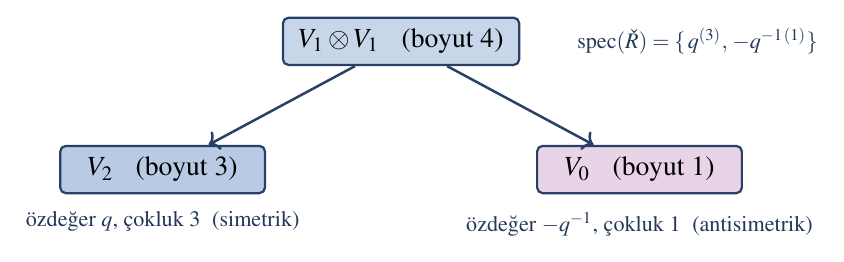
\includegraphics[width=0.82\linewidth]{figures/tikz_spec-1.png}
\caption{\textbf{Şekil 8.3} Örgülü Ř'nin spektral ayrışması, V1⊗ V1=V2⊕ V0
Clebsch--Gordan ayrışımıyla aynıdır. Özdeğer çoklukları doğrudan alt-temsil
boyutlarını verir (\texttt{R\_check\_eigenvalues}).}
\label{fig:spec}
\end{figure}

\section{Düğüm Değişmezleriyle Bağlantı (İleri Görü)}

Hecke skein bağıntısı, check R ile üretilen Bn temsilinin aslında Hecke
cebri Hn(q) üzerinden çarpanlandığını söyler. Bu temsile bir Markov izi
uygulandığında ortaya çıkan değişmez, tam olarak sl2 tipindeki
\emph{Jones polinomudur}~\cite{Jones}. Jones polinomunun somut hesabı bu tezin kapsamı
dışında tutulmuştur; ancak ona giden yapısal basamaklar --- örgü bağıntısı ve
Hecke özdeşliği (Önerme~8.2 ve~8.3) --- burada kurulmuş
ve seçilen matris modeli üzerinde doğrulanmıştır. Jones polinomunun tam
hesaplanması ve Markov izi bu çalışmanın kapsamı dışındadır.

\chapter{GLq(2|1) için Graded Yang--Baxter Doğrulaması}

Tezin ayırt edici hesaplamalı katkısı bu bölümdedir: kuantum süpergrup
GLq(2|1) için literatürde verilen R-matrisinin graded Yang--Baxter
denklemini gerçekten sağladığı, sembolik matris doğrulamasıyla bütün girdiler
düzeyinde ortaya konur.

\section{Motivasyon}

Salih Çelik ve Sultan A.\ Çelik \cite{CelikGL21}, GLq(2|1) kuantum süpergrubunu
V=C^2|1 süper vektör uzayı üzerindeki bir R-matrisinden RTT
yöntemiyle inşa eder. Burada amaç, Çelik ve Çelik'in çalışmasında~\cite{CelikGL21} verilen 9× 9 R-matrisini
kodlayıp graded Yang--Baxter denkleminin matris girdileri düzeyinde sağlandığını
bağımsız biçimde doğrulamaktır.

Bu doğrulamanın el ile yapılması zahmetlidir: denklem 27× 27 matrislerin
çarpımına dayanır ve uzun, tekrarlı yapısı nedeniyle işaret/sıralama hatalarına
açıktır. Dahası --- birazdan görüleceği gibi --- graded yapı, sıradan bir
matris hesabının ötesinde parite bilgisinin doğru taşınmasını da gerektirir. Bu
iki neden, hesabı açık baz, açık parite ve açık süper permütasyon matrisiyle
Python/SymPy üzerinde modellemeyi doğal kılar.

Baz sıralaması $e_1e_1,\,e_1e_2,\,e_1e_3,\,e_2e_1,\,e_2e_2,\,e_2e_3,\,
e_3e_1,\,e_3e_2,\,e_3e_3(kısacae_ie_j:=e_i\otimes e_j$) alındığında, kodlanan
9× 9 R-matrisi şudur:
\begin{equation}\label{eq:Rgl21}
R=\begin{pmatrix}
1 & 0    & 0 & 0      & 0 & 0    & 0      & 0      & 0\\
0 & q^2  & 0 & 1-q^2  & 0 & 0    & 0      & 0      & 0\\
0 & 0    & q & 0      & 0 & 0    & 1-q^2  & 0      & 0\\
0 & 0    & 0 & 1      & 0 & 0    & 0      & 0      & 0\\
0 & 0    & 0 & 0      & 1 & 0    & 0      & 0      & 0\\
0 & 0    & 0 & 0      & 0 & q    & 0      & 1-q^2  & 0\\
0 & 0    & 0 & 0      & 0 & 0    & q      & 0      & 0\\
0 & 0    & 0 & 0      & 0 & 0    & 0      & q      & 0\\
0 & 0    & 0 & 0      & 0 & 0    & 0      & 0      & q^2
\end{pmatrix}.
\end{equation}
Girdilerin yalnızca dört farklı türü (1, q, q^2, 1-q^2) ve seyrek yerleşimi,
paketin ürettiği Şekil~9.1'de renk kodlu olarak görülebilir.

\begin{figure}[h]
\centering

\includegraphics[width=0.74\textwidth]{R_gl21_structure-1.png}
\caption{\textbf{Şekil 9.1} (9.1) R-matrisinin girdi-tipi haritası (\texttt{R\_matrix\_GLq21}
çıktısı). Köşegen q/q^2 terimleri ile köşegen-dışı 1-q^2 ``karışım''
terimleri açıkça ayrışır; bu seyreklik, 27× 27 ve 81× 81
yerleşimlerin neden hâlâ hesaplanabilir kaldığını da açıklar.}
\label{fig:rgl21}
\end{figure}

\section{Graded Yapı ve Süper Permütasyon}

Süper vektör uzayı V=C^2|1'in baz vektörleri parite (derece)
taşır:
\[
p(e_1)=0,\qquad p(e_2)=0,\qquad p(e_3)=1,
\]
yani e1,e2 çift, e3 tektir. Graded ortamda iki faktörün yer değiştirmesi,
klasik takasla aynı olamaz: süper cebirde iki tek (odd) nesne yer değiştirirken
Koszul işaret kuralı gereği bir eksi işareti ortaya çıkar. Bu, V⊗ V
üzerindeki \emph{süper permütasyon} matrisiyle kodlanır:
\[
P(e_i\otimes e_j)=(-1)^{p(e_i)p(e_j)}\,e_j\otimes e_i.
\]
Dolayısıyla P, klasik permütasyon matrisinden yalnızca tek--tek (odd--odd)
bileşendeki işaret değişimiyle ayrılır. Bu küçük görünen ayrıntı belirleyicidir:
R13 operatörü süper permütasyon yardımıyla kurulduğundan, işaret yanlış
modellenirse R13 ve onunla birlikte tüm graded Yang--Baxter hesabı
matematiksel olarak anlamını yitirir. Kod, bu parite bilgisini doğrudan matris
düzeyine taşır:

\begin{lstlisting}[style=pyblock,caption={V ⊗ V uzerinde super permutasyon matrisi}]
def super_permutation_matrix(parity):
    d = len(parity)
    P = sp.zeros(d*d, d*d)
    for i in range(d):
        for j in range(d):
            # Koszul isareti: yalniz tek--tek bilesende -1
            sign = -1 if parity[i] and parity[j] else 1
            P[j*d + i, i*d + j] = sign
    return P
\end{lstlisting}

GLq(2|1) için \texttt{parity}=[0,0,1] verildiğinden eksi işareti yalnızca
e3⊗ e3 bileşeninde, yani P[8,8]=-1 girdisinde belirir; kalan tüm
girdiler klasik takasla aynıdır (Şekil~9.2).

\begin{figure}[h]
\centering
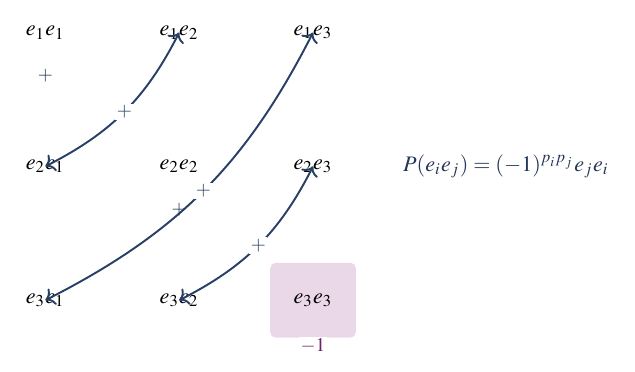
\includegraphics[width=0.82\linewidth]{figures/tikz_superperm-1.png}
\caption{\textbf{Şekil 9.2} Süper permütasyon P, V⊗ V bazı üzerinde bir takas: köşegen-dışı
çiftler işaretsiz (+) yer değiştirir, köşegen sabit kalır; tek istisna
odd--odd köşesi e3e3'tür (-1, vurgulu). Klasik takastan tek fark budur.}
\label{fig:superperm}
\end{figure}

\section{R12, R13, R23 Yerleşimleri}

Çelik ve Çelik'in makalesindeki~\cite{CelikGL21} R-matrisi V⊗ V üzerinde etki eden 9× 9 bir
operatördür. Üçlü çarpım V⊗ V⊗ V üzerinde komşu faktör
yerleşimleri doğrudandır:
\[
R_{12}=R\otimes I_3,\qquad R_{23}=I_3\otimes R.
\]
Komşu olmayan birinci ve üçüncü faktöre etki eden R13 ise ancak süper
permütasyonla eşlenerek kurulabilir:
\[
R_{13}=(P\otimes I_3)\,R_{23}\,(P\otimes I_3).
\]
İşte parite bilgisinin hesaba sızdığı yer tam da budur: R13, R23'ün
süper permütasyonla ``iki kez döndürülmüş'' hâlidir ve P'deki tek eksi işaret
doğrudan bu operatöre geçer. Şekil~9.3 bu üç yerleşimi iplik
diyagramı olarak karşılaştırır: R12 ve R23 komşu ipliklere doğrudan
oturur, R13 ise 1.\ ve 3.\ iplikleri süper permütasyonla komşulaştırıp
R'yi uygulayıp tekrar açan bir konjugasyonla kurulur.

\begin{figure}[h]
\centering
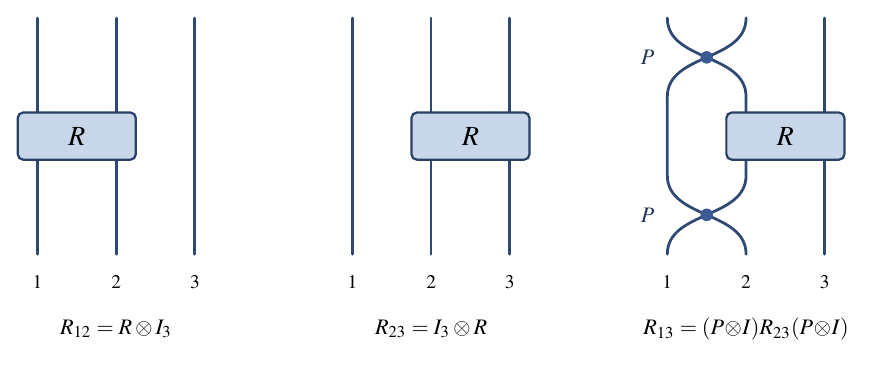
\includegraphics[width=0.82\linewidth]{figures/tikz_place-1.png}
\caption{\textbf{Şekil 9.3} Üç faktörlü uzayda Rij yerleşimleri. Komşu yerleşimler (R12,R23)
basit Kronecker gömmeleridir; uzak yerleşim R13 ise süper permütasyon P
ile konjugasyon gerektirir --- elle takibi en zor olan, bu çalışmada
otomatikleştirilen adım.}
\label{fig:place}
\end{figure}

Bu fikir tek bir yerleşime özgü değildir. Pakette, R'yi herhangi bir
V^⊗ n uzayında istenen (i,j) faktör çiftine taşıyan genel bir gömme
fonksiyonu tanımlıdır.

\paragraph{Önerme 9.1 (Konjugasyonla genel yerleşim).}\label{prop:embed}
d=dim V ve Sk, k ile k+1 faktörlerini değiş-tokuş eden komşu graded
takas operatörü olsun (Sk=I^⊗ k⊗ P⊗ I^⊗(n-k-2)).
i<j için V^⊗ n üzerindeki Ri,j operatörü, komşu yerleşim
Ri,i+1=I^⊗ i⊗ R⊗ I^⊗(n-i-2)'in ardışık
konjugasyonuyla elde edilir:
\[
R_{i,j}=S_{j-1}\cdots S_{i+1}\,R_{i,i+1}\,S_{i+1}\cdots S_{j-1}.
\]
Bu konjugasyon graded işaretleri doğru taşır; j=i+1 için ifade basit Kronecker
gömmesine indirgenir.


Bu önermenin kod karşılığı doğrudan ve test edilebilirdir:

\begin{lstlisting}[style=pyblock,caption={R-matrisini V^⊗ n icinde (i,j) faktorlerine gomme}]
def embed_R_in_tensor_power(R, positions, tensor_power, parity):
    i, j = positions                       # sifirdan baslayan indisler, i < j
    d, n = len(parity), tensor_power
    # Komsu yerlesim R_{i, i+1}
    op = _kron_list([_eye_pow(d, i), R, _eye_pow(d, n - i - 2)])
    # Ikinci indisi konjugasyonla i+1'den j'ye tasi (graded takas)
    for k in range(i + 1, j):
        S_k = _adjacent_swap(parity, n, k)
        op = S_k * op * S_k
    return op
\end{lstlisting}

V⊗ V⊗ V için (i,j)=(0,2) seçilince bu fonksiyon yukarıdaki
R13 formülünü birebir yeniden üretir; V^⊗ 4'te ise altı
yerleşimin hepsi aynı çağrıyla otomatik kurulur.

\section{Sıfır-Kalıntı Yöntemi}

Graded Yang--Baxter denklemi yine
\[
R_{12}R_{13}R_{23}=R_{23}R_{13}R_{12}
\]
biçimindedir. Önceki bölümlerle aynı şablon izlenerek kalıntı matrisi
\[
Y(q)=R_{12}R_{13}R_{23}-R_{23}R_{13}R_{12}
\]
kurulur; bu 27× 27 boyutlu bir matristir. SymPy ile yapılan girdi-bazlı
sadeleştirme,
\[
Y(q)_{ij}=0,\qquad 1\leq i,j\leq 27,
\]
yani matrisin tamamının sıfır olduğunu verir. Hesabın çekirdeği şudur:

\begin{lstlisting}[style=pyblock,caption={GLq(2|1) icin graded Yang--Baxter kalintisi}]
def graded_yang_baxter_residual_GLq21(q_sym=q):
    # GL_q(2|1) graded Yang--Baxter kalinti matrisi (27x27)
    R12 = R12_GLq21(q_sym)
    R13 = R13_GLq21(q_sym)   # super permutasyonla kurulur
    R23 = R23_GLq21(q_sym)
    return R12*R13*R23 - R23*R13*R12

def graded_yang_baxter_holds_GLq21(q_sym=q):
    Y = graded_yang_baxter_residual_GLq21(q_sym)
    # All 27x27 entries symbolically zero?
    return all(sp.simplify(x) == 0 for x in Y)
\end{lstlisting}

Bu fonksiyon 27× 27 kalıntıyı oluşturur ve her girdiyi sembolik olarak
sıfıra indirger. Sonuç Şekil~9.4'de görselleştirilmiştir: eşitliğin
iki tarafı --- R12R13R23 ve R23R13R12 --- tıpatıp aynı
sıfır-olmayan örüntüye sahiptir (her birinde 729 girdiden 58'i sıfırdan
farklı), farkları Y(q) ise tümüyle boştur. Böylece seçilen baz sıralaması ve
p=(0,0,1) parite konvansiyonu altında graded Yang--Baxter eşitliğinin matris
girdileri düzeyinde sağlandığı hem sembolik hem görsel olarak doğrulanır.

\begin{figure}[h]
\centering

\includegraphics[width=\textwidth]{ybe_products_27-1.png}
\caption{\textbf{Şekil 9.4} Graded Yang--Baxter denkleminin iki tarafının 27× 27
sıfır-olmayan örüntüleri özdeştir; kalıntı $Y(q)=R_{12}R_{13}R_{23}-
R_{23}R_{13}R_{12}tüm729$ girdide sıfırdır
(\texttt{graded\_yang\_baxter\_residual\_GLq21}).}
\label{fig:ybe27}
\end{figure}

\section{Dört Faktörlü Genişleme}

Yöntemin tek bir denkleme bağlı kalmadığını göstermek için, R-matrisinin
V^⊗ n üzerine genel yerleşimini üreten bir fonksiyon da yazılmıştır.
Örneğin V^⊗ 4 üzerinde
\[
R_{12}, R_{13}, R_{14}, R_{23}, R_{24}, R_{34}
\]
operatörleri 81× 81 matrisler olarak elde edilebilir. Bu boyut tesadüfi
değildir: süpergrup hesapları hızla büyür (3^3=27, 3^4=81) ve elle takibi
neredeyse olanaksız hâle gelir; sembolik altyapı ise Önerme~9.1'in
şablonunu boyuttan bağımsız biçimde uygular. V^⊗ 4'ün altı yerleşimi
ve aralarındaki ilişkiler, K4 tam grafiği üzerinden okunabilir
(Şekil~9.5): grafiğin altı kenarı altı Rij operatörüne, dört
üçgeni dört lokal Yang--Baxter kontrolüne, ayrık kenar çifti ise uzak
komütativiteye karşılık gelir. Bu sayede hem uzak komütativite
\[
R_{12}R_{34}=R_{34}R_{12}
\]
hem de dört ayrı üçlü altblok için lokal graded Yang--Baxter kontrolleri
\[
R_{ab}R_{ac}R_{bc}=R_{bc}R_{ac}R_{ab}
\]
otomatik olarak yürütülür (Çizelge~9.1).

\begin{figure}[h]
\centering
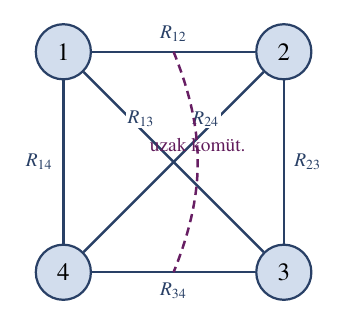
\includegraphics[width=0.82\linewidth]{figures/tikz_k4-1.png}
\caption{\textbf{Şekil 9.5} V^⊗ 4 yerleşimlerinin K4 grafiği: altı kenar altı Rij,
dört üçgen (1,2,3,1,2,4,1,3,4,2,3,4) dört lokal Yang--Baxter
kontrolü, ayrık kenar çifti (12)--(34) ise uzak komütativitedir.}
\label{fig:k4}
\end{figure}

Dört üçlü altblok kontrolü tek bir fonksiyonda toplanır:

\begin{lstlisting}[style=pyblock,caption={V^⊗ 4 icindeki dort uclu icin lokal YBE kontrolu}]
def local_ybe_on_four_tensor_GLq21(q_sym=q):
    Rij = all_Rij_GLq21(4, q_sym)          # six 81x81 placements
    result = {}
    for a, b, c in combinations(range(4), 3):   # (0,1,2),(0,1,3),(0,2,3),(1,2,3)
        Rab, Rac, Rbc = Rij[(a, b)], Rij[(a, c)], Rij[(b, c)]
        residual = Rab*Rac*Rbc - Rbc*Rac*Rab
        result[(a, b, c)] = _is_zero_matrix_symbolic(residual)
    return result
\end{lstlisting}

\begin{table}[h]
\centering
\small
\caption{\textbf{Çizelge 9.1} V^⊗ 4 üzerindeki yerleşimler ve otomatik kontroller (tümü
81× 81; \texttt{all\_Rij\_GLq21}, \texttt{local\_ybe\_on\_four\_tensor\_GLq21},
\texttt{braid\_far\_commutativity\_residual\_GLq21}).}
\label{tab:vtensor4}
\begin{tabularx}{\textwidth}{@{}l l X@{}}
\toprule
Kontrol & İlgili operatörler & Anlamı \\
\midrule
Yerleşimler & R12,R13,R14,R23,R24,R34 & K4'ün altı kenarı \\
\addlinespace[1pt]
Lokal YBE × 4 & üçlüler (a,b,c) & RabRacRbc=RbcRacRab \\
\addlinespace[1pt]
Uzak komütativite & R12,R34 & ayrık kenarlar komüte eder \\
\bottomrule
\end{tabularx}
\end{table}

\section{Metodolojik Katkı}

Bu bölümün asıl kazanımı yöntemseldir. Literatürde verilen GLq(2|1)
R-matrisinin graded Yang--Baxter denklemine ilişkin uzun ve elle yürütülen
hesabı, burada açık kaynaklı, test edilebilir ve yeniden üretilebilir bir
sembolik doğrulama prosedürüne dönüşmüştür. Klasik kâğıt-kalem hesabının
güvenilirliği ile bilgisayar destekli sembolik cebrin ölçeklenebilirliği,
parite bilgisini matris düzeyine taşıyan tek bir çerçevede birleşir.

\chapter{Klasik, Kuantum ve Birim Kök Limitleri}\label{sec:limits}

Son hesaplamalı katkı, aynı Vn temsilini üç farklı asimptotik rejimde yan
yana koyarak ``kuantize etmenin'' somut anlamını göstermektir. Kuantum gruplar
bu üç rejimde nitel olarak farklı davranır; bunu tek bir temsil üzerinde
izlemek, deformasyonun nereye dokunduğunu açıkça ortaya koyar.

\section{(L1) Klasik Limit q → 1}

Cartan elemanını şu limitle geri kazanırız:
\[
  h := \lim_{q \to 1} \frac{K - 1}{q - 1}.
\]
Köşegen olduğu için h'nin k. girişi
limq → 1 (q^n-2k - 1)/(q - 1) = n - 2k, yani klasik
sl2 ağırlığıdır.

\paragraph{Önerme 10.1 (Seçilen temsillerde sayısal doğrulama).}\label{thm:classical}
Vn için, h = limq→ 1 (K-1)/(q-1) ile tanımlanan operatörün
köşegen girişleri n, n-2, n-4, ..., -n'dir; ve aynı limit
limq→ 1 [E,F] = h olur.


Doğrulama, V1, V2, V3, V4 için \path{tests/test_limits.py}
içindeki \path{test_classical_commutator_equals_h} testi ile
yapılmıştır.

\section{(L2) Genel q}

Çalışmanın büyük kısmının yürüdüğü asıl kuantum rejim budur. K-özdeğerleri
q^n, q^n-2, ..., q^-n, E-katsayıları ise [k]q[n-k+1]q
biçimindedir. Burada q birim kökü olmadığından temsil teorisi klasik durumun
``düzgün'' bir deformasyonudur: Vn indirgenemez kalır, dört bağıntı ve dokuz
Hopf aksiyomu sembolik q üzerinde sağlanır.

\section{(L3) Birim Kök q^N = 1}

q bir N. primitif birim kökü zeta = e^2pi i/N ile değerlendirildiğinde
[N]q=0 olur ve genel-q resmi köklü biçimde değişir. E^N, F^N ve
K^2N merkezîleşir; bazı [k]q[n-k+1]q katsayıları sıfırlandığından
daha önce indirgenemez olan kimi Vn temsilleri parçalanabilir hâle gelir.
Yani deformasyonun ``zararsız'' göründüğü genel rejimden, temsil teorisinin
yeniden kurulmasını gerektiren bir rejime geçilir.

\paragraph{Örnek 10.2 (Sayısal gözlem).}
N = 4 alalım, yani q = i. V2 üzerinde E-matris katsayıları
[1]q[2]q ve [2]q[1]q formundadır. Burada
\[
  [2]_q = q + q^{-1} = i + i^{-1} = 0
\]
olduğundan, hesaplama E = 0_3 verir:
\[
  E\big|_{q=i} = \begin{pmatrix} 0 & 0 & 0 \\ 0 & 0 & 0 \\ 0 & 0 & 0 \end{pmatrix}.
\]
Yani V2, q = i'de yapısal olarak \emph{çöker} ve genel q
durumundakinden farklı, indirgenebilir bir Uq(sl2)|_q=i-modül hâline
gelir. Bu olgu \path{tests/test_limits.py::test_root_of_unity_V2_at_q4_singular}
ile sayısal olarak doğrulanmıştır.


Bunun teorik anlamı, ``küçük kuantum grup'' uq(sl2)'nin (Lusztig)
ortaya çıkışıdır: birim kökte Uq(sl2)'nin sonlu boyutlu indirgenemez
temsilleri sınıflanması tamamen değişir, blok yapısı belirir, ve kuantum
gruplar konformal alan teorisi ile bağlantı kurar.

\section{(L4) Kristal Limit q → 0}

Üçüncü teorik bölümde tartışılan kristal taban, aslında q→ 0 limitine
karşılık gelir. Bu rejimde tekil matris katsayıları ıraksasa da Vn'in
kombinatoryal gölgesi --- kristal B(n) ---
\[
  b_0 \xrightarrow{\tilde f} b_1 \xrightarrow{\tilde f} \dots
   \xrightarrow{\tilde f} b_n
\]
yolu olarak ayakta kalır; tilde f, F-eyleminin tek bir oka indirgenmiş
hâli, tilde e ise tersidir. Pakette bu yapı \texttt{quantum\_group/crystal.py}
modülünde bir grafik nesnesi olarak kurulur ve görselleştirilir.

\section{Üç Limitin Karşılaştırması (V2 örneği)}

\begin{table}[h]
\centering
\small
\caption{\textbf{Çizelge 10.1} V2 temsilinin üç limit rejimindeki karşılaştırması.}
\label{tab:limits}
\begin{tabularx}{\textwidth}{@{}lXXX@{}}
\toprule
& Klasik (q → 1) & Genel q & Birim kök (q^4 = 1) \\
\midrule
K-özdeğerleri & 1, 1, 1 & q^2, 1, q^-2 & -1, 1, -1 \\
h-özdeğerleri & 2, 0, -2 & --- & --- \\
E-girdileri & 2, 2 & [1]q[2]q, [2]q[1]q & 0, 0 \\
İndirgenemez mi? & Evet & Evet & \textbf{Hayır} \\
Boyut & 3 & 3 & 3 \\
\bottomrule
\end{tabularx}
\end{table}

Böylece tek bir temsil, kuantum grubun ``q parametresinin üç ayrı hayatını''
aynı çerçevede gözler önüne serer.

\chapter{Sonuç ve Öneriler}

Bu çalışmada Uq(sl2) kuantum grubu ile GLq(2|1) kuantum süpergrubu, aynı
sembolik sıfır-kalıntı doğrulama çekirdeği üzerinden ele alındı. Elde edilen
sonuçlar şöyle özetlenebilir:

\begin{itemize}[leftmargin=*]
  \item \textbf{Uq(sl2) temsilleri}: Sonlu boyutlu Vn temsilleri açık
        matrislerle uygulandı; E,F,K,K^-1 operatörleri ve ağırlık verileri
        tek bir temsil nesnesinde toplandı.
  \item \textbf{Bağıntılar ve Hopf yapısı}: Dört (R1)--(R4) bağıntısı ve Hopf
        yapısı, seçilen sonlu boyutlu temsiller üzerinde sembolik
        sıfır-kalıntı testleriyle doğrulandı.
  \item \textbf{Tensör teorisi}: Vm ⊗ Vn üzerinde eş-çarpımdan gelen
        eylem kuruldu; Clebsch--Gordan ayrışımının en yüksek ağırlık vektörleri
        q-deforme katsayılarıyla elde edildi.
  \item \textbf{R-matrisi ve örgü bağıntıları}: V1 ⊗ V1 üzerinde
        R-matrisi, kuantum Yang--Baxter denklemi, örgü bağıntısı ve Hecke
        bağıntısı hesaplamalı olarak kontrol edildi.
  \item \textbf{Graded durum}: Salih Çelik ve Sultan A.\ Çelik'in
        GLq(2|1) R-matrisi için graded Yang--Baxter denklemi, parite
        uyumlu süper permütasyonla kurulan R13 yerleşimi kullanılarak
        27× 27 kalıntı matrisinin tüm girdileri düzeyinde doğrulandı.
  \item \textbf{Yeniden üretilebilirlik}: Raporlanan kontroller
        \texttt{pytest} testlerine bağlandı; şekiller ve PDF çıktısı depo
        içindeki betikler ve \texttt{Makefile} hedefleriyle yeniden üretilebilir
        hâle getirildi.
\end{itemize}

Uq(sl2) tarafındaki kazanç, klasik temsil teorisini R-matrisi/örgü altyapısıyla
tek bir test edilebilir pakette buluşturmaktır. GLq(2|1) tarafında ise asıl
katkı yöntemseldir: literatürdeki uzun graded Yang--Baxter hesabı, açık baz,
açık parite ve açık süper permütasyon üzerinden yeniden üretilebilir bir sembolik
prosedüre dönüşür. Sonuçların tamamı --- \texttt{tests/} birim testleri,
\texttt{requirements.txt} bağımlılıkları, LaTeX kaynağı ve üretilen PDF --- depo
klonlanarak yeniden elde edilebilir.

Bu yaklaşım, yüksek boyutlu Yang--Baxter tipi hesapların elle yürütülen
cebirsel manipülasyonlardan, test edilebilir ve yeniden üretilebilir sembolik
doğrulama prosedürlerine taşınabileceğini göstermektedir.

\paragraph{İleri çalışma yönleri.}
\begin{enumerate}[leftmargin=*]
  \item \emph{Jones polinomu hesaplaması}: bu çalışmadaki örgü temsilini Markov
        izi ile birleştirerek küçük düğümlerin (trefoil, sekiz-düğüm) Jones
        polinomunu hesaplama.
  \item \emph{Yüksek rank}: Uq(sln) ve genel Cartan tipi için aynı
        altyapının genelleştirilmesi.
  \item \emph{Küçük kuantum grup}: uq(sl2)'nin birim kökünde tam
        temsil teorisinin ve blok yapısının inşası.
  \item \emph{Crystal tensör çarpımı}: B(m) ⊗ B(n) kristal
        kuralının uygulanması ve klasik Clebsch--Gordan ile karşılaştırılması.
  \item \emph{Gauss ayrışımı ve Hopf süpercebir}: GLq(2|1) için
        ilgili makaledeki~\cite{CelikGL21} Gauss ayrışımı, üst/alt üçgensel alt süpergruplar, RTT
        bağıntıları ve Hopf süpercebir eşlemelerinin kodla doğrulanması.
\end{enumerate}

% ======================= KAYNAKLAR (APA, alfabetik) =======================
\FloatBarrier

\begin{thebibliography}{99}
\setlength{\itemsep}{6pt}

\bibitem{ChariPressley}
Chari, V., Pressley, A., (1994). \emph{A Guide to Quantum Groups}, Cambridge University Press, Cambridge.

\bibitem{CelikGL21}
Çelik, S., Çelik, S.~A., (2021). ``A New Quantum Supergroup and its Gauss Decomposition'', \emph{Reports on Mathematical Physics}, 88(2), 259--272.

\bibitem{Drinfeld}
Drinfeld, V.~G., (1986). ``Quantum Groups'', \emph{Proceedings of the International Congress of Mathematicians}, Berkeley, ABD.

\bibitem{HK}
Hong, J., Kang, S.-J., (2002). \emph{Introduction to Quantum Groups and Crystal Bases}, American Mathematical Society, Providence.

\bibitem{Jimbo}
Jimbo, M., (1985). ``A q-difference Analogue of U(g) and the Yang--Baxter Equation'', \emph{Letters in Mathematical Physics}, 10, 63--69.

\bibitem{Jones}
Jones, V.~F.~R., (1985). ``A Polynomial Invariant for Knots via von Neumann Algebras'', \emph{Bulletin of the American Mathematical Society}, 12, 103--111.

\bibitem{Kashiwara}
Kashiwara, M., (1991). ``On Crystal Bases of the q-analogue of Universal Enveloping Algebras'', \emph{Duke Mathematical Journal}, 63, 465--516.

\bibitem{Kassel}
Kassel, C., (1995). \emph{Quantum Groups}, Graduate Texts in Mathematics 155, Springer, New York.

\bibitem{KS}
Klimyk, A., Schmüdgen, K., (1997). \emph{Quantum Groups and Their Representations}, Springer, Berlin.

\bibitem{pytest}
Krekel, H. vd., (2004). \emph{pytest documentation}, \url{https://docs.pytest.org/}, 3 Haziran 2026.

\bibitem{Lusztig}
Lusztig, G., (1993). \emph{Introduction to Quantum Groups}, Birkhäuser, Boston.

\bibitem{SymPy}
Meurer, A. vd., (2017). ``SymPy: Symbolic Computing in Python'', \emph{PeerJ Computer Science}, 3, e103.

\end{thebibliography}

\addcontentsline{toc}{chapter}{KAYNAKLAR}


\clearpage
\phantomsection
\addcontentsline{toc}{chapter}{EKLER}
\appendix
\renewcommand{\thechapter}{\Alph{chapter}}
\renewcommand{\thesection}{\thechapter.\arabic{section}}
\renewcommand{\thefigure}{\thechapter.\arabic{figure}}
\renewcommand{\thetable}{\thechapter.\arabic{table}}
\titleformat{\chapter}[hang]
  {\normalfont\fontsize{17.5}{21}\bfseries}{EK~\thechapter}{12pt}{}

\chapter{Kurulum, Çalıştırma ve Yeniden Kullanım Kılavuzu}

Bu ek, bu teze eşlik eden kod deposunun kurulumu, test edilmesi, şekillerinin
yeniden üretilmesi ve ileride genişletilmesi için temel adımları özetler. Depo
adresi \url{https://github.com/TerekliTahaBerk/quantum-groups} şeklindedir.

\section{Depo Yapısı}

Depo, bu tezdeki sembolik hesaplamaları ve belge üretim sürecini ayrı
dizinlerde tutacak biçimde düzenlenmiştir:
\begin{itemize}[leftmargin=*]
  \item \texttt{quantum\_group/}: sembolik hesaplamaları uygulayan Python
        paketi.
  \item \texttt{tests/}: \texttt{pytest}~\cite{pytest} tabanlı test takımı.
  \item \texttt{thesis/}: LaTeX kaynağı, üretilen PDF dosyası ve şekil
        dosyaları.
  \item \texttt{thesis/figures/}: şekil üretim betiği ve çıktı şekilleri.
  \item \texttt{notebooks/}: keşif amaçlı Jupyter defteri.
  \item \texttt{main.py}: kısa kullanım gösterimi.
  \item \texttt{Makefile}: test, şekil üretimi, PDF derleme ve demo için
        kolaylık komutları.
  \item \texttt{requirements.txt}: Python bağımlılıkları.
  \item \texttt{MANUSCRIPT\_CODE\_MAPPING.md}: tezdeki başlıklar ile
        depo uygulaması arasındaki eşleme.
\end{itemize}

\Needspace{10\baselineskip}
\section{Ortamın Hazırlanması}

\Needspace{9\baselineskip}
Python ortamı aşağıdaki komutlarla hazırlanabilir:
\begin{lstlisting}[style=bashblock]
git clone https://github.com/TerekliTahaBerk/quantum-groups.git
cd quantum-groups
python3 -m venv .venv
source .venv/bin/activate
python3 -m pip install --upgrade pip
python3 -m pip install -r requirements.txt
\end{lstlisting}

\Needspace{5\baselineskip}
Windows üzerinde sanal ortam etkinleştirme komutu şöyledir:
\begin{lstlisting}[style=bashblock]
.venv\Scripts\activate
\end{lstlisting}

Bağımlılıkların rolleri kısaca şöyledir: SymPy~\cite{SymPy} sembolik cebir ve matris
sadeleştirme için, NetworkX kristal grafiği ve grafik yardımcıları için,
Matplotlib şekil üretimi için, pytest test takımı için, Jupyter ise defter
tabanlı keşif çalışmaları için kullanılır.

\Needspace{10\baselineskip}
\section{Testlerin Çalıştırılması}

\Needspace{5\baselineskip}
Tüm test takımı aşağıdaki komutla çalıştırılır:
\begin{lstlisting}[style=bashblock]
python3 -m pytest tests/ -q
\end{lstlisting}

\Needspace{5\baselineskip}
Aynı işlem \texttt{Makefile} üzerinden de çağrılabilir:
\begin{lstlisting}[style=bashblock]
make test
\end{lstlisting}

\Needspace{7\baselineskip}
Belirli test dosyaları ayrı ayrı çalıştırılabilir:
\begin{lstlisting}[style=bashblock]
python3 -m pytest tests/test_r_matrix.py -q
python3 -m pytest tests/test_supergroup_gl21.py -q
python3 -m pytest tests/test_tensor.py -q
\end{lstlisting}

\texttt{test\_r\_matrix.py}, R-matrisini, kuantum Yang--Baxter denklemini,
örgü bağıntısını ve Hecke bağıntısını kontrol eder.
\texttt{test\_supergroup\_gl21.py}, GLq(2|1) R-matrisini, süper
permütasyonu, graded Yang--Baxter denklemini ve seçili tensör-kuvvet
yerleşimlerini kontrol eder. \texttt{test\_tensor.py} ise tensör çarpımı
eylemini ve Clebsch--Gordan örneklerini denetler. Bu testler, tezdeki açık
matris modelleri üzerinde kullanılan sembolik kontrolleri tekrar çalıştırmak
için verilmiştir.

\Needspace{9\baselineskip}
\section{Demo Çalıştırma}

\Needspace{5\baselineskip}
Kısa kullanım gösterimi şu komutla çalıştırılır:
\begin{lstlisting}[style=bashblock]
python3 main.py
\end{lstlisting}

\Needspace{5\baselineskip}
\texttt{Makefile} eşdeğeri:
\begin{lstlisting}[style=bashblock]
make demo
\end{lstlisting}

Bu demo, paketin temel kullanımını göstermek içindir; ayrıntılı sembolik
kontroller \texttt{tests/} dizinindeki testlerde yer alır.

\Needspace{9\baselineskip}
\section{Şekillerin Yeniden Üretilmesi}

\Needspace{5\baselineskip}
Tezdeki şekiller aşağıdaki betikle yeniden üretilebilir:
\begin{lstlisting}[style=bashblock]
python3 thesis/figures/generate_figures.py
\end{lstlisting}

\Needspace{5\baselineskip}
\texttt{Makefile} eşdeğeri:
\begin{lstlisting}[style=bashblock]
make figures
\end{lstlisting}

Betik, çıktı dosyalarını \texttt{thesis/figures/} dizinine yazar. Depodaki
üretilen başlıca şekil dosyaları şunlardır:
\begin{itemize}[leftmargin=*]
  \item \texttt{R\_sl2\_V1.pdf}
  \item \texttt{R\_gl21\_structure.pdf}
  \item \texttt{ybe\_products\_27.pdf}
\end{itemize}

Figürlerde matematiksel semboller mümkün olduğunca Matplotlib mathtext ile
üretilmiştir; Türkçe açıklamalar ise çoğunlukla LaTeX başlıklarında ve şekil
açıklamalarında tutulmuştur.

\Needspace{8\baselineskip}
\section{PDF'in Derlenmesi}

\Needspace{5\baselineskip}
PDF derleme için önerilen hedef şudur:
\begin{lstlisting}[style=bashblock]
make pdf
\end{lstlisting}

Mevcut \texttt{Makefile} tanımına göre \texttt{make pdf}, önce şekilleri yeniden
üretir, ardından \texttt{thesis/thesis.tex} dosyasını derler. Derleme sonunda
kalıcı olarak yalnızca tezin ana PDF dosyası tutulur:
\begin{itemize}[leftmargin=*]
  \item \texttt{thesis/Quantum Grup Yapılarının Python Ortamında Modellenmesi.pdf}
\end{itemize}

\Needspace{8\baselineskip}
\section{Gelecek Genişletmeler İçin Notlar}

Yeni bir hesaplama başlığı eklenirken, ilgili uygulama kodunun
\texttt{quantum\_group/} altında ayrı bir modülde veya mevcut uygun modülde
tutulması; buna karşılık gelen testlerin \texttt{tests/} altında açık ve hedefli
test dosyalarıyla verilmesi önerilir. Yeni şekiller için üretim mantığı
\texttt{thesis/figures/generate\_figures.py} içinde tutulabilir veya aynı dizinde
ayrı betiklere ayrılabilir; çıktı dosyalarının adları LaTeX kaynağındaki
\texttt{\textbackslash includegraphics} çağrılarıyla tutarlı olmalıdır. Teze
eklenen yeni hesaplama iddiaları için \texttt{MANUSCRIPT\_CODE\_MAPPING.md}
dosyasındaki eşlemenin güncellenmesi, ileride bakım ve yeniden kullanım
açısından yararlıdır.

\Needspace{16\baselineskip}
\chapter{Test Eşlemesi}

Her doğrulama ekseni, ilgili kod modülü ve birim test dosyasıyla
Çizelge~B.1'te eşlenmiştir.

\begin{table}[H]
\centering
\footnotesize
\caption{\textbf{Çizelge B.1} Doğrulama eksenleri, kod modülleri ve test dosyaları.}
\label{tab:tests}
\begin{tabularx}{\textwidth}{@{}>{\raggedright\arraybackslash}p{0.24\textwidth}X>{\raggedright\arraybackslash}p{0.30\textwidth}@{}}
\toprule
Doğrulama & Kod Modülü & Test Dosyası \\
\midrule
Uq(sl2) bağıntıları & \texttt{relations.py} & \texttt{test\_relations.py} \\
Hopf aksiyomları & \texttt{hopf.py} & \texttt{test\_hopf.py} \\
Temsiller ve kristaller & \texttt{representations.py}, \texttt{crystal.py} & \texttt{test\_representations.py} \\
Clebsch--Gordan & \texttt{tensor.py} & \texttt{test\_tensor.py} \\
R-matrisi/QYBE & \texttt{r\_matrix.py} & \texttt{test\_r\_matrix.py} \\
GLq(2|1) graded YBE & \texttt{supergroup\_gl21.py} & \texttt{test\_supergroup\_gl21.py} \\
Limit analizleri & \texttt{limits.py} & \texttt{test\_limits.py} \\
\bottomrule
\end{tabularx}
\end{table}


% ======================= ÖZGEÇMİŞ =======================
\clearpage
\chapter{ÖZGEÇMİŞ}
\addcontentsline{toc}{chapter}{ÖZGEÇMİŞ}

\noindent
\textbf{Kişisel Bilgiler}\\[4pt]
\begin{tabularx}{\textwidth}{@{}p{4cm}X@{}}
Adı Soyadı      & : Taha Berk TEREKLİ \\
Bölümü          & : Matematik Bölümü \\
Üniversite      & : Yıldız Teknik Üniversitesi, Fen-Edebiyat Fakültesi \\
\end{tabularx}

\vspace{0.6cm}
\noindent
\textbf{Eğitim}\\[4pt]
\begin{tabularx}{\textwidth}{@{}p{4cm}X@{}}
Lisans & : Yıldız Teknik Üniversitesi, Matematik Bölümü \\
\end{tabularx}

\vspace{0.6cm}
\noindent
\textbf{İlgi Alanları}\\[4pt]
Kuantum gruplar, temsil teorisi, Yang--Baxter denklemi, sembolik hesaplama
(Python/SymPy), bilgisayar cebiri.

\vspace{0.6cm}
\noindent
\textbf{Tez Çalışmasına İlişkin}\\[4pt]
Bu bitirme tezi kapsamında geliştirilen \texttt{quantum\_group} Python paketi ve
ilgili test takımı, açık kaynak olarak
\url{https://github.com/TerekliTahaBerk/quantum-groups} adresinde
yayımlanmıştır.

\end{document}
